\documentclass[conference]{IEEEtran}
\usepackage[utf8]{inputenc}
\usepackage[T1]{fontenc}
\usepackage{amsfonts}
%\usepackage{amsthm}
\usepackage{makeidx}  % allows for indexgeneration
\usepackage{amsmath}
\usepackage{mathtools}
\usepackage{verbatim}
\usepackage{float}
\usepackage{graphicx}
\usepackage{times}  
\usepackage[lined, boxed, linesnumbered]{algorithm2e}
\usepackage{array}
\usepackage{tikz}
\usepackage{lscape}

\usetikzlibrary{positioning,arrows}
%\tikzset{m/.style={ellipse,draw,fill=gray!40,minimum size=20},outer sep=5pt}

%\usepackage{fancyhdr}
%\usepackage[nofancy]{svninfo}
%\usepackage{multicol}
\usepackage{ifdraft}
\usepackage[all]{xy}
\usepackage{caption}
\usepackage{subcaption}
\usepackage{cite}
\usepackage{marginnote}
\usepackage{todonotes}

\title{A Branch and Price Algorithm for the Single-Path Virtual Network Embedding Problem}
\author{\IEEEauthorblockN{Leonardo F.S. Moura}
\IEEEauthorblockA{Computer Science Department,\\  Federal University of Rio Grande do Sul\\
Porto Alegre, Brazil \\
lfsmoura@inf.ufrgs.br}
\and
\IEEEauthorblockN{Luciana S. Buriol}
\IEEEauthorblockA{Computer Science Department,\\  Federal University of Rio Grande do Sul\\
Porto Alegre, Brazil \\
buriol@inf.ufrgs.br}
}

\newtheorem{proposition}{Proposition}
\newtheorem{corollary}{Corollary}
\newtheorem{theorem}{Theorem}[section]
\newtheorem{lemma}{Lemma}[section]
\newcommand{\todoc}[1]{\todo[color=red!20, bordercolor=white]{#1}}
\newcommand{\todoi}[1]{\todo[inline,color=red!20, bordercolor=white]{#1}}
\begin{document}

\maketitle

% Networks : abstract
% A short abstract (200 words maximum) as well as 4-6 keywords are required. It should be complete and self-contained, giving the scope and emphasizing the main conclusions, results, or significance of the work described.

\begin{abstract}
Virtualization is a growing trend in the implementation of cloud computing architectures.
The Virtual Network Embedding problem (VNEP) is one of the challenges in the virtualization of physical networks. 
This work shows that finding a feasible solution for this problem is NP-Hard.
However it can be solved up to optimality in practice by exploiting the problem structure.
%This work shows that the problem is NP-Hard, as well as hard to approximate.
%Due to its hardness, most works present heuristic algorithms or relaxations of the problem.
%However, the relaxation of the integer linear programming formulation presented in the literature yields a low quality lower bound. 
%In this work we use a flow-based formulation of the problem and solve the relaxation using a
%column generation approach. 
%This method results in high quality lower bounds obtained in short time, as the computational experiments show.
%This suggests that it can be successfully embedded in a branch \& price method for providing optimal solutions for the VNEP.
We present a Branch \& Price algorithm applied to instances of different topologies and sizes.
The experimental results suggest that the proposed algorithm is superior to the ILP model solved by CPLEX.

\end{abstract}

\begin{IEEEkeywords}
Virtual Network Embedding, Column Generation, Integer Linear Programming, Branch \& Price.
\end{IEEEkeywords}

\section{Introduction}
Network virtualization was proposed for overcoming the problem of ossification of the Internet, a way to facilitate the evolution of its protocols~\cite{Anderson2005}. 
In virtualized environments, multiple networks can simultaneously use the same physical structure in a transparent way. By creating a new layer of abstraction over the physical networks, new protocols can be tested on heterogeneous experimental architectures~\cite{Anderson06geni}.
Likewise, service providers can offer customized services or co-location for expanded network presence~\cite{Feamster:2007}. Virtualization is being used in practice~\cite{Carapinha:2009,Anderson06geni} and it is considered the main enabling technology for cloud computing.

The Virtual Network Embedding Problem (VNEP) is central to achieve network virtualization. 
It consists in mapping virtual networks with heterogeneous architectures on physical infrastructures. 
Virtual nodes are mapped into physical substrate nodes and virtual links are mapped into paths in the physical substrate network. 
Additionally, physical resources are finite and must be used judiciously: nodes have a processing capacity and links have a bandwidth limit.
The main objective of the VNEP is to minimize the use of the underlying resources such as bandwidth, while respecting the mapping constraints.

As network virtualization is not yet a mature field, problems are still being defined and classified.
Different classifications and more information about different constraints of virtualization problems are found in \cite{Fischer:2011,Chowdhury2010,FischerSurvey}.
There are several variations of the VNEP such as mapping virtual networks individually as they arrive~\cite{Chowdhury2010}, or mapping a batch of virtual network requests simultaneously~\cite{Houidi:2011,Guerzoni:2014}.
Physical nodes and links can be restricted to host a limited number of virtual nodes and links, or certain virtual links can have a location restriction.
Some applications have security restrictions, that limit the subset of physical nodes and links that can be used for mapping~\cite{Buriol:2012}.
Additional constraints can also be present such as delay~\cite{infuhr:2011}, efficient use of energy~\cite{Botero:2012}, and redundancy~\cite{Shamsi:2008}. 
This work captures the core of those constraints into a VNEP definition that is both hard and generic.

Some works, such as \cite{Yu2008,hu:2013}, allow path splitting, i.e., they allow virtual links to be mapped to multiple paths in the substrate network, effectively splitting data between two or more channels in the physical substrate.
Even though path-splitting allows the use of simple algorithms for link mapping, in certain contexts, such as teleconferencing, path splitting cannot be implemented~\cite{Barnhart:2000}.
Path splitting can incur in extra costs for infrastructure providers, and can violate security constraints.
Furthermore, current network technology do not generally support path splitting \cite{Guerzoni:2014}.
For all those reasons, this work focuses on the Single-Path VNEP.

The VNEP is hard to solve in practice. In this work we show that even finding a feasible solution is NP-Hard. 
The problem is harder to solve than other related problems such as Virtual Private Network (VPN) Design, which consists in reserving part of the network resources to allow a subset of nodes to communicate \cite{Gupta:2001}.
In the VNEP, the mapping of nodes is not fixed, greatly increasing the solution space.

Due to the difficulty of solving the VNEP, few exact algorithms are proposed in the literature.
For most practical purposes, heuristic algorithms can provide good suboptimal solutions for the problem.
Still, exact algorithms serve as a comparison or baseline to evaluate heuristic algorithms.
Moreover, they can be practical for specific cases, such as for small virtual networks or physical networks with abundant resources.

A backtrack algorithm based on subgraph isomorphism detection is presented in~\cite{Lischka:2009}. In that study, both nodes and edges are mapped simultaneously, so that infeasible node mappings can be detected quickly and discarded.
Most exact algorithms are based on Integer Linear Programming (ILP) models. 
The first of such algorithms is proposed in~\cite{Chowdhury:2012} for the multiple-path VNEP.
In~\cite{Houidi:2011,Guerzoni:2014}, ILP models that map multiple virtual networks simultaneously are proposed.
A single-path model is presented in~\cite{Alkmim2013}.
Some of these works present a rounding scheme to obtain integer solutions from the relaxation of the integer models. Nonetheless, heuristic methods or rounding schemes do not provide a guarantee of finding feasible solutions for the VNEP. 
On the experimental side, only small instances are solved up to optimality with a general purpose solver within a reasonable amount of time.
A natural attempt in solving this problem efficiently is by using problem specific exact algorithms, instead of general purpose solvers.
Developing specialized cuts for integer models or devising better bounds on the optimal solution are important ingredients to improve exact algorithms. 
Column generation approaches were proposed for the multiple-path VNEP~\cite{hu:2013}, and for the single-path VNEP with multiple requests~\cite{Jarray2012}.

Our previous work showed that the flow-based model produces better lower bounds than the compact model \cite{Moura:2014}.
Therefore it is better suited to be integrated into a Branch \& Bound algorithm.
%In \cite{hu:2013}, a flow-based model with path splitting is presented. 
In this work we propose a column generation algorithm for the single-path VNEP, based on a flow-based model proposed by~\cite{hu:2013}, but adapted to single-paths.
%Since the number of paths in graphs grows exponentially with the size of the graph, a column generation algorithm is applied with the aim of generating a high quality lower bound for the problem. 
%The linear relaxation of that model results in a high quality lower bound than the linear relaxation of the flow formulation.
%We consider the case of mapping a single virtual network, and each physical node is restricted to host a single virtual link.
We embedded the column generation into a Branch \& Price algorithm for producing integer solutions for the problem.
To the best of our knowledge this is the first problem-specific exact algorithm presented for the VNEP.
We compared results with the ILP model solved with CPLEX when both approaches are applied to instances of different sizes and topologies.
The proposed Branch \& Price algorithm presented better results in terms of time and solution cost.

% old outline
%The paper is structured as follows: Section~\ref{sec:prob} formalizes the Virtual Network Embedding Problem, overviews its complexity and present the classic ILP Model. 
%In Section~\ref{sec:flow} the flow-based model is introduced. A column generation and a the Branch \& Price algorithms are presented in Sections~\ref{sec:cg} and Sections~\ref{sec:bp}, respectively.  
%Section~\ref{sec:results} presents experimental results and their analysis. Finally, Section~\ref{sec:conclusion} concludes this work, presenting suggestions for future lines of research.

The paper is structured as follows: Section~\ref{sec:prob} formalizes the Virtual Network Embedding Problem, overviews its complexity, presents the classic ILP Model and the new flow-based model. A column generation is presented in Section~\ref{sec:cg} and in Section~\ref{sec:bp} a Branch \& Price algorithm is presented.
Section~\ref{sec:results} presents experimental results and their analysis. Finally, Section~\ref{sec:conclusion} concludes this work, presenting suggestions for future research extensions.


%%%%%%%%%%%%%%%%%%%%%%%%%%%%%%%%%%%%%%%%%%%%%%%%%%%%%%%%
\section{Virtual Network Embedding Problem}
\label{sec:prob}
A VNEP instance has as input a virtual network and physical substrate network. The physical substrate is represented by an undirected graph $G^S = (V^S,E^S)$ with a CPU capacity of $C_{s}$ for each physical node $s \in V^S$ and a bandwidth capacity $B_{e}$ for each edge $e \in E^S$. The virtual network is represented by a undirected graph $G^V = (V^V,E^V)$ along with a demand $C_{v}$ for each virtual node $v \in V^V$, and a bandwidth demand of $B_{k}$ for each virtual link $k \in E^V$. 

The objective of the proposed problem is to find a feasible mapping of the virtual nodes and links onto the physical network with minimal cost. 
A feasible mapping is a pair of functions $(f_v, f_e)$: A mapping of nodes $f_v: V^V \rightarrow V^S$ and a mapping of links $f_{e=(w,u)}: E^V \rightarrow P$, where $P$ is the set of paths in the substrate graph with endpoints $f_v(w)$ and $f_v(u)$.
Each virtual node has to be mapped into a single substrate node with enough CPU capacity to host it. A substrate node can host at most one virtual node. Each virtual link $(w,u) \in E^V$ has to be mapped to a path in the physical graph between the nodes $f_v(w)$ and $f_v(u)$. An edge can host several virtual links, but the sum of their demands could not surpass the capacity of the edge. The cost of a mapping is the amount of bandwidth used in the physical network by the mapping.

Figure~\ref{fig:input} presents an instance of the problem composed of a physical network with four nodes and a virtual network with three nodes. 
Edges and nodes are labelled with their capacities or demands. 
%Next to each node label is the capacity or demand of the node.
The optimal mapping is shown in Figure~\ref{fig:mapping}. 
%Since the substrate node $d$ is the only one with enough capacity to host $p3$, 
The optimal solution is to map node $a$ to $C$, $b$ to $A$, and $c$ to $B$;
the virtual link  $(a,b)$ is mapped to $C-B-A$, and the virtual link $(b,c)$ is mapped to $A-B$. The cost of this solution is $50$.


%\tikzstyle{every node}=[draw, ellipse, minimum size=100pt,align=center]
\begin{figure}[h]
  \centering
  \begin{subfigure}[h]{0.45\linewidth}
  \centering    
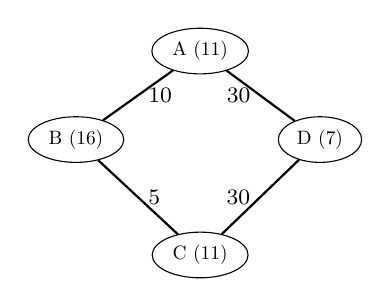
\begin{tikzpicture}
\usetikzlibrary{arrows}
\usetikzlibrary{shapes}
\tikzstyle{every node}=[draw, ellipse, minimum size=10pt,align=center,scale=0.7]
\node at (0,0)(1){A (11)};
\node[below left=1cm of 1](2){B (16)};
\node[below right=1cm of 1](4){D (7)};
\node[below=2cm of 1](3){C (11)};
\path[every node/.style={font=\footnotesize},thick]
    (1) edge node[right] {10} (2)
	edge node[left] {30} (4)
    (2) edge node[right] {5} (3)
    (4) edge node[left] {30} (3);
\end{tikzpicture}
  \subcaption{Physical Network}\label{fig:Physical}
  \end{subfigure}  
  \begin{subfigure}[h]{0.53\linewidth}
  \centering
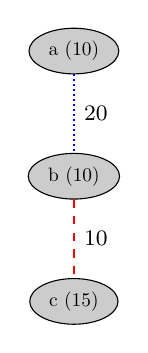
\begin{tikzpicture}
\usetikzlibrary{arrows}
\usetikzlibrary{shapes}
\tikzstyle{every node}=[draw, ellipse, fill=gray!40, minimum size=10pt, align=center, scale=0.7]
\node at (0,0)(1){a (10)};
\node[below=1cm of 1](2){b (10)};
\node[below=1cm of 2](3){c (15)};
\path[every node/.style={font=\footnotesize},thick]
    (1) edge[blue,densely dotted] node[right,color=black] {20} (2)
    (2) edge[red,thick,dashed] node[right,color=black] {10} (3);
\end{tikzpicture}
  \subcaption{Virtual Network}\label{fig:Virtual}
  \end{subfigure}   
  \caption{An input instance for the VNEP.}\label{fig:input}   
\end{figure}


\begin{figure}[h]
  \centering
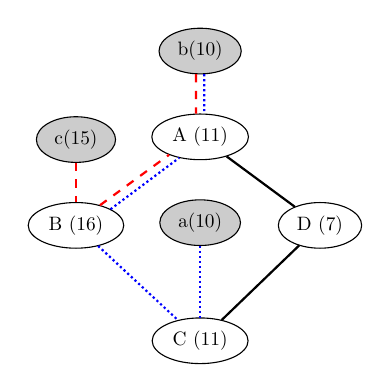
\begin{tikzpicture}
\usetikzlibrary{arrows}
\usetikzlibrary{shapes}
\tikzstyle{every node}=[draw, ellipse, minimum size=10pt,align=center,scale=0.7]
\node[fill=gray!40] at (0,0)(6){b(10)};
\node[below=0.5cm of 6] (1){A (11)};
\node[below left=1cm of 1](2){B (16)};
\node[below right=1cm of 1](4){D (7)};
\node[below=2cm of 1](3){C (11)};
\node[fill=gray!40, below=0.5cm of 1] (5){a(10)};
\node[fill=gray!40, above=0.5cm of 2] (7){c(15)};
\path[every node/.style={font=\footnotesize},thick]
    (5) edge[blue,densely dotted] node [] {} (3)
    (7) edge[red,dashed] node [] {} (2)
    (1) edge node [] {} (4)
    (2) edge[blue,densely dotted] node [] {} (3)
    (4) edge node [] {} (3);
  \draw[blue,thick,densely dotted] (2.25) -- (1.-135);
  \draw[red,thick,dashed] (2.40) -- (1.-150);
  \draw[blue,thick,densely dotted] (6.-80) -- (1.80);
  \draw[red,thick,dashed] (6.-100) -- (1.100);
\end{tikzpicture}
  \caption{Optimal solution for instance of Figure~\ref{fig:input}.\label{fig:mapping}}   
\end{figure}


In Subsection~\ref{sec:complexity} we characterize the complexity of the single-path VNEP.
That Subsection can be skipped without loss of continuity.
Next, Subsection~\ref{sec:ILPmodel} introduces a general ILP Model for the problem.

\subsection{Complexity}
\label{sec:complexity}
%Several heuristics were developed for the VNEP, but none of them is guaranteed to find a feasible solution. 
We show in this section that %there could not exist an efficient algorithm that always finds a feasible solution 
%(not necessarily the optimal solution) unless $P=NP$, and then there is no approximation algorithm for the VNEP.
%Initially we show that 
the VNEP problem is NP-Hard by a reduction from the Bin Packing Problem (BPP), which is a classical NP-Complete problem.
The VNEP was previously shown to be NP-Hard by a reduction from the Unsplittable Flow Problem~\cite{Yu2008}, 
but by the reduction from the BPP we further show it does not exist an algorithm that is guaranteed to generate a feasible solution unless P=NP, and then VNEP cannot be approximated.

The Bin Packing Problem has as input a set~$N$ of items and a bin size of capacity~$B$.  Each item~$i$ has a weight~$w_{i} \leq B$. The goal is to fit all items using the minimum number of bins, respecting their capacities. The decision version asks if it is possible to fit all items in at most $k$ bins.


Any instance $I$ of the BPP can be transformed into an instance of the VNEP through the procedure $\phi$, which generates a virtual and physical graphs as described next.
%First we show that $\phi$ is polynomial in the size of $N$, then we show that a polynomial algorithm that finds a feasible solution for the VNEP provides a polynomial algorithm for the B\&P. 
%By the transformation, a physical substrate graph is created with $2|N| + 2k$ nodes and $2|N|k + k$ edges, and a virtual network graph is created with $2|N|$ nodes and $2n - 1$ edges, as described next. 
%This new instance is created in such a way that there is a feasible solution for the VNEP instance $\phi(I)$ iff there is also a solution for instance $I$. Therefore an algorithm that finds any feasible solution for the VNEP solves B\&P.

\textbf{Virtual Network:} For each item $i \in N$, two nodes are created: one with demand three and another with demand two. 
Those nodes are linked with virtual links with bandwidth $w_{i}$. 
Moreover, nodes corresponding to items $i$ and $i+1$ for every $i < |N|$ are linked to assure the connectivity of the network.
Their demand is not important and are set to zero.

\textbf{Physical Substrate Network:} For each item $i \in N$ two nodes are created, one with capacity three and another with capacity two. 
Furthermore, $2k$ nodes are created with capacity one. 
For convenience, let us call nodes with capacity three the upper nodes, nodes with capacity two the lower nodes, and nodes with capacity one the middle nodes, in the physical and virtual networks.
Each upper node is linked with $k$ middle nodes, the rest of the $k$ middle nodes is linked with all lower nodes. 
Each of the~$k$ middle nodes linked with the upper nodes are linked with one single middle node which is linked to the lower nodes. 
Capacities of all edges are set to~$B$, the bin size.

An example of this transformation is show in Figures~\ref{fig:transsub} and~\ref{fig:transvir}. 
The original BPP consists of three items of weights three, four, and eight, and $B=8$. 
The value of $k$ in the decision version is set to two. 
A solution is given by mapping the virtual links with weights three and four on physical edges on the left-central, 
and the other virtual link of weight eight into the edge on the right-central.

\begin{figure}
  \centering
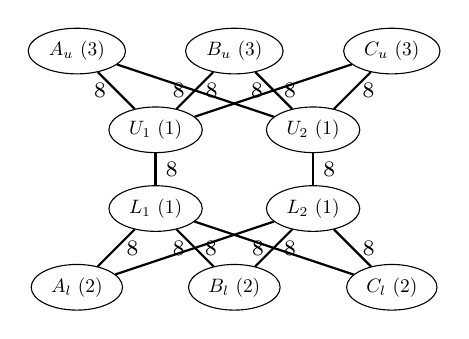
\begin{tikzpicture}
\usetikzlibrary{arrows}
\usetikzlibrary{shapes}
\usetikzlibrary{graphs}
\tikzstyle{every node}=[draw, ellipse, minimum size=10pt,align=center,scale=0.7]
\node at (0,3)(1){$A_{u}$ (3)};
\node at (2,3)(2){$B_{u}$ (3)};
\node at (4,3)(3){$C_{u}$ (3)};
\node at (1,2)(4){$U_{1}$ (1)};
\node at (3,2)(5){$U_{2}$ (1)};
\node at (1,1)(6){$L_{1}$ (1)};
\node at (3,1)(7){$L_{2}$ (1)};
\node at (0,0)(8){$A_{l}$ (2)};
\node at (2,0)(9){$B_{l}$ (2)};
\node at (4,0)(10){$C_{l}$ (2)};
%  \draw (1) -- (4) node [below]{8};

\path[every node/.style={font=\footnotesize},thick]
    (1) edge node[left] {8} (4) 
    (1) edge node[right] {8} (5)
    (2) edge node[left] {8} (4)
    (2) edge node[right] {8} (5)
    (3) edge node[left] {8} (4)
    (3) edge node[right] {8} (5)
    (4) edge node[right] {8} (6)
    (5) edge node[right] {8} (7)
    (8) edge node[right] {8} (6)
    (8) edge node[right] {8} (7)
    (9) edge node[left] {8} (6)
    (9) edge node[right] {8} (7)
    (10) edge node[left] {8} (6)
    (10) edge node[right] {8} (7);
\end{tikzpicture}
  \caption{Substrate Graph resulted from transformation $\phi$.}\label{fig:transsub}
\end{figure}

\begin{figure}
  \centering
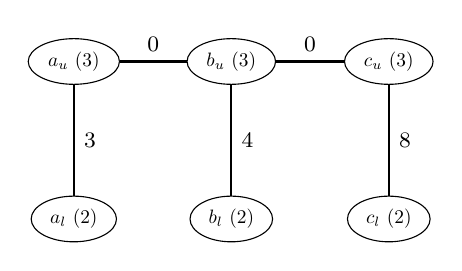
\begin{tikzpicture}
\usetikzlibrary{arrows}
\usetikzlibrary{shapes}
\usetikzlibrary{graphs}
\tikzstyle{every node}=[draw, ellipse, minimum size=10pt,align=center,scale=0.7]
\node at (0,2)(1){$a_{u}$ (3)};
\node at (2,2)(2){$b_{u}$ (3)};
\node at (4,2)(3){$c_{u}$ (3)};
\node at (0,0)(8){$a_{l}$ (2)};
\node at (2,0)(9){$b_{l}$ (2)};
\node at (4,0)(10){$c_{l}$ (2)};
%  \draw (1) -- (4) node [below]{8};

\path[every node/.style={font=\footnotesize},thick]
    (1) edge node[right] {3} (8)
    (2) edge node[right] {4} (9)
    (3) edge node[right] {8} (10)
    (1) edge node[above] {0} (2)
    (2) edge node[above] {0} (3);
\end{tikzpicture}
  \caption{Virtual Graph resulted from transformation $\phi$.}\label{fig:transvir}
\end{figure}

\begin{lemma} \label{lem:reduction}
  Any Bin Packing instance can be reduced to an instance of the Virtual Network Embedding Problem through procedure $\phi$.
\end{lemma}

\begin{proof}
There are~$n$ virtual nodes with demand three and~$n$ physical nodes with capacity three, therefore any feasible solution would map all virtual upper nodes to physical upper nodes. Likewise for physical and virtual nodes with capacity and demand two.
Hence, in the instance~$\phi(I)$ there is always a feasible mapping of the nodes.
Moreover, each of the~$n$ edges has to be mapped to a single path in the substrate graph between the upper nodes and the lower nodes.
Additionally, every path has to contain at least one edge between the middle nodes.
Those edges represent bins.
Mapping virtual links to those edges is tantamount to fit items in a bin.
%Hence, if a solution for $\phi(I)$ is given, a solution for $I$ can be obtained by selecting the first of the middle edges (the edges that link the middle nodes) in the $n$ paths.
%Moreover, if there is any feasible mapping for $\phi(I)$, the answer for the B\&P decision version is YES. 
%Therefore, if a polynomial algorithm exists that solves $\phi(I)$, we can use it to compute the answer to $I$ in polynomial time.
\end{proof}


\begin{lemma} \label{lem:transpol}
  The transformation $\phi(I)$ is polynomial in $|N|$.
\end{lemma}

\begin{proof}
The transformation $\phi$ creates two graphs, one with $2|N| + 2k$ nodes and $2|N|k + k$ edges and another with $2|N|$ nodes and $2n - 1$ edges. 
As $k < |N|$, and every item fits into a single bin, the size of the VNEP instance is limited polynomially by $|N|$, the number of items of $I$.
\end{proof}

\begin{lemma} \label{lem:polapp}
  If there exists a polynomial time algorithm that finds a feasible solution for $\phi(I)$, there is a polynomial time algorithm that finds a feasible solution for $I$.
\end{lemma}

\begin{proof}
All virtual nodes with demand three have to be mapped to substrate nodes with capacity three.
If one of the nodes of demand two is mapped to a substrate node of capacity three, there will be an unmapped virtual node of capacity three. 
Likewise, for nodes of capacity two.
%as there are only $|N|$ substrate nodes with capacity two, every one of the $|N|$ virtual nodes with demand two will be mapped to a substrate node of capacity two. 
Therefore there is always a feasible node mapping for $\phi(I)$. 
Note that the mapping order is not important: any virtual node with demand $x$ can be mapped to any physical node with capacity $x$.

\paragraph{If there is a feasible mapping for the virtual network of $\phi(I)$, the answer to I is YES}
Given a feasible mapping $M$, all virtual edges are mapped to a path in the substrate graph. 
Let $p_{i}$ be the path for which the virtual link~$i$, corresponding to the item~$i$, was mapped to. 
Let $j$ be the first substrate edge in $p_{i}$ that links the middle nodes. The edge~$j$ corresponds to the bin~$j$. Thus a solution for $I$ can be constructed if item~$i$ is allocated into bin~$j$. 
Since the capacity of all edges are not surpassed, the $k$~bins can hold the $|N|$~items.

\paragraph{If the answer for I is YES, there is a feasible mapping for $\phi(I)$}
Suppose that there is a configuration of the items into $k$ bins.
A solution for $\phi(I)$ can be constructed from a solution for $I$.
Suppose any feasible mapping $M$ of nodes for the virtual network (as it was shown before, there always exists a feasible mapping of nodes).
Let $f_{M}(u)$ be the substrate node for which the virtual node $u$ is mapped. 
Every virtual link $(u,v)$ corresponding to the item $i$ is mapped to the path $(f_{M}(u), x)$, $(x,y)$, $(y,f_{M}(v))$, where $(x,y)$ is the substrate edge corresponding to the bin $j$ for which the item $j$ was allocated in the solution for $I$.
Since the sum of the items in a bin $j$ does not exceed the capacity $B$, every virtual link can be mapped in the physical graph.
\end{proof}

\begin{lemma} \label{lem:cert}
  VNEP is an NP problem
\end{lemma}

\begin{proof}
  A solution for a VNEP instance I can be verified in polynomial time in the size of the instance. For every virtual node $u$ it suffices to check if the physical node $f_v(u)$ has enough capacity to host it, for every virtual link $(u,w)$ it suffices to check the path $p = f_e(u,w)$ is indeed a path (every adjacent edge shares one endpoint), and for every physical edge $e$, if all the links that are mapped in $e$ do not surpass its capacity.
\end{proof}

\begin{theorem} \label{th:npcomplete}
  VNEP is an NP-Complete problem.
\end{theorem}

\begin{proof}
The hardness of the VNEP problem follows from Lemmas~\ref{lem:reduction}-\ref{lem:cert}. 
\end{proof}

\begin{corollary} \label{co:nopoly}
  There is no polynomial time algorithm that finds a feasible solution for VNEP, unless $P=NP$.
\end{corollary}

\begin{proof}
  Suppose there is a polynomial time algorithm that finds a feasible solution (not necessarily optimal) for VNEP. From~\ref{lem:polapp}, it follow that there is a polynomial algorithm for solving BPP\@. 
  But this is only possible if $P = NP$.
\end{proof}

Corollary~\ref{co:nopoly} implies that there is probably no time efficient approximation algorithm for VNEP, since such an algorithm would provide a polynomial time algorithm to solve BPP.

\subsection{A Compact ILP Model}
\label{sec:ILPmodel}
Most exact algorithms for the VNEP are based on ILP models. 
An ILP model for VNEP with path-splitting was presented in~\cite{Chowdhury2009}, 
while~\cite{Alkmim:2011} consider single-path variant of the problem.
We present an ILP model inspired by these two previous models, but for a basic version of the single-path VNEP problem.
Let the decision variables~$x_{vs} = 1$ iff the substrate node $s$ hosts the virtual node $v$. And let $y_{vwst} = 1$ iff the physical link $(s,t)$ hosts the virtual link $(v,w)$.

%\scriptsize
\begin{align}
     \min & \sum\limits_{(s,t) \in E^{S}} \sum\limits_{(v,w) \in E^{V}} B_{vw}~ y_{vwst} & \nonumber \\
    s.t. & \sum\limits_{v \in V^{V}} C_{v} x_{vs} \leq C_{s}                                   & \forall s \in V^{S}  \label{eq:flowcap} \\
         & \sum\limits_{s \in V^{S}} x_{vs} = 1                                                & \forall v \in V^{V}  \label{eq:flowvirone}\\
         & \sum\limits_{v \in V^{V}} x_{vs} \leq 1                                             & \forall s \in V^{S} \label{eq:flowsubone} \\
         & \sum\limits_{t \in V^{S}} ( y_{vwst} - y_{vwts}) = x_{vs} - x_{ws} & \forall (v,w) \in E^{V}, \nonumber \\ 
         &                                                                    & s \in V^{S} \label{eq:flowflow} \\
         & \sum\limits_{(v,w) \in E^{V}} B_{vw}  y_{vwst} \leq B_{st}                 & \forall (s,t) \in E^{S} \label{eq:flowbandwidth} \\
         & x_{vs} \in \{0,1\}                                                                  & \forall v \in V^{V}, \nonumber \\
         &                                                                                      & s \in V^{S} \\
         & y_{klmn} \in \{0,1\}                                                         & \forall (k,l) \in E^{V}, \nonumber \\
         &                                                                                 & (m,n) \in E^{S}
\end{align} 

The objective function minimizes the amount of bandwidth used. 
Constraints~\eqref{eq:flowcap} ensure that the substrate capacities are not surpassed. 
Constraints~\eqref{eq:flowvirone} enforce that every virtual node is mapped to a substrate node, while~\eqref{eq:flowsubone} enforce that every substrate node hosts at most one virtual node. 
Constraints~\eqref{eq:flowflow}
ensure that every virtual link is mapped to a path into the substrate graph. Finally, constraints~\eqref{eq:flowbandwidth} ensure that the bandwidth capacities of physical edges are not surpassed.

Although \cite{Chowdhury:2012} and \cite{Alkmim2013} present ILP models for the VNEP, they deemed impractical to solve the models optimally and presented rounding schemes applied to the relaxed solutions in order to obtain integer solutions.
However, rounding does not guarantee to find a feasible mapping.
Moreover, the relaxation of this model does not produce a good lower bound for the problem since it generates a zero-cost solution.

\begin{proposition}
There is always a solution with cost zero to the compact model.
\end{proposition}

\begin{proof}
If every $x_{vs}$ is set to~$1 / |V^S| $, all constraints are respected and the left hand side of Constraints~\eqref{eq:flowflow} is zero. 
Therefore all variables $y_{vwsj}$ can be set to zero.
Hence, the cost of the optimal solution for the relaxed problem is always zero, resulting in a trivial lower bound.
\end{proof}

The model presented in the next section provides better bounds and exploits better the problem structure.


\subsection{Flow-based Model}
\label{sec:flow}

VNEP can be modeled in terms of paths in the auxiliary graph. % instead of the hosting relationship between physical edges and virtual links such as the compact model presented in Section~\ref{sec:ILPmodel}.
%As stated in that section, the lower bound obtained from the relaxation of this model is not informative.
%Column generation models have more columns but generally result in better lower bounds.
%Such models can better exploit specific information about the problem domain.
%We present in this section a CG model defined in terms of feasible paths in the physical network.
Two sets of decision variables are used. For each $v \in V^{V}$ and $s \in V^{S}$, the variable $x_{vs} \in \{0,1\}$ is set to one iff the substrate node $s$ hosts the virtual node~$v$. 
Likewise, for each path $p$ in the set of all paths $P$, the variable $z_{p} \in \{0,1\}$ is set to one if the path is used in the VNEP. 
For each path~$p$, the input data $\delta_{e,p}$ is one if the physical edge~$e$ is in the path~$p$, and zero otherwise.
For each virtual link $k=(v,w) \in V^V$, $P^k$ is the set of all simple paths in the substrate graph whose endpoints have enough CPU capacity to host $v$ and $w$, and whose links have enough capacity to host $k$.
The set of Constraints~\eqref{eq:flowcap} of the compact model can be omitted because only paths that attend this constraint are part of the model.
The objective function is the minimization of the total bandwidth used by the virtual network. 
If a path $p$ serves a virtual link $k$, the cost of this path $c_{p}$ is defined as the number of physical edges in the path.
The flow-based model for the single-path VNEP is presented below:

\begin{align}
  \min  & \sum\limits_{k \in E^{V}}\sum\limits_{p \in P^k}  c_{p} B_k z_{p}        \nonumber \\
  s.t.  & \sum\limits_{s \in V^{S}} x_{v,s} = 1                                  & \forall v \in V^{V} \label{eq:virone} \\
        & \sum\limits_{v \in V^{V}} x_{v,s} \leq 1                               & \forall s \in V^{S} \label{eq:subone} \\
        & \sum\limits_{p \in P^{k}} z_{p} = 1                                    & \forall k \in E^{V} \label{eq:virdemone} \\
        & \sum\limits_{k \in E^{V}}\sum\limits_{p \in P^{k}} \delta_{e,p} B_{k} z_{p} \leq B_{e} & \forall e \in E^{S} \label{eq:bandwidth} \\
        & \sum\limits_{k \in E^{V}}\sum\limits_{p \in P^k : (v,s) \in p} z_{p} \leq M x_{v,s} & \forall v \in V^{V}, s \in V^{S} \label{eq:onlyoneaux}\\
        &  x_{v,s} \in \{0,1\}  & \forall v \in V^{V}, s \in V^{S} \nonumber \\
        & z_{p} \in \{0,1\}    & \forall p \in {P} \nonumber
\end{align}

Constraints~\eqref{eq:virone} ensure that all virtual nodes are mapped. Each substrate node can host at most one virtual node~\eqref{eq:subone}.
Constraints~\eqref{eq:virdemone} state that all virtual links have to be mapped to a single path in the substrate graph.
Constraints~\eqref{eq:bandwidth} ensure that the bandwidth constraints are not violated.
Finally, let M be the greatest degree of the virtual network, Constraints~\eqref{eq:onlyoneaux} enforce that only one auxiliary edge is used for each virtual node.

%This model has one variable for each possible feasible path in the physical graph.
%Since the number of paths in a graph grows exponentially with the size of the graph,
%it is impractical to solve this model using standard algorithms such as Simplex Algorithm.
%A Column Generation algorithm is used to solve the relaxation of this model.


%%%%%%%%%%%%%%%%%%%%%%%%%%%%%%%%%%%%%%%%%%%%%%%%%%%%%%%%
\section{A column generation algorithm}
\label{sec:cg}

Column generation is a mathematical programming technique proposed by Dantzig and Wolfe \cite{Dantzig:1960} 
to solve models with a large number of variables.
These ``large'' models usually provide better bounds on the optimal integer solutions than compact models, and this is the case for the VNEP.
%The restricted master problem, comprised of a subset of variables (columns), is solved at each iteration of the CG.

Although the number of variables in a large model grows exponentially with the size of the instance,
the number of nonzero variables in a solution is small.
The column generation algorithm takes advantage of that.
A Restricted Master Problem (RMP) comprised of a limited set of columns is solved.
More columns are generated and added to the RMP by solving a subproblem (pricing), until no more columns improving the solution.
%When no more columns are generated that could improve the solution, the optimal solution is found.

The proposed column generation algorithm is summarized in Algorithm~\ref{alg:cg}.
Initially, in Line~\ref{alg:artificial}, artificial variables are added to the RMP so that there is always a feasible solution.
That process is explained in Section~\ref{sec:initcol}.
The RMP is solved in Line~\ref{alg:solve}.
The pricing problem is solved in lines~\ref{alg:pricingbegin} through~\ref{alg:pricingend},
and it is further explained in Section~\ref{sec:pricing}
The pricing problem generates columns to be added to the RMP, and when no more columns are generated, the algorithm stops.

\begin{algorithm}
%\scriptsize
$P' = \emptyset$\;
Add artificial variables to the model such that model is feasible\; \label{alg:artificial}
\Repeat{No paths were added to $P'$}
  {Solve model with limited set of columns $P'$\; \label{alg:solve}
  \ForEach{Virtual link $(u,v) \in E^{V}$ \label{alg:pricingbegin} }
    {Construct auxiliary graph $A$ using dual variables\; \label{alg:aux}
    Find minimum cost $u$-$v$-path $p$ in $A$ with reduced cost $r_{p}$\; \label{alg:findpaths}
    \If{$r_{p} < 0$}
      {Add path to $P'$\;}
    } \label{alg:pricingend}
  }
\eIf{All artificial variables are equal to zero\label{alg:feascond}}
  {The problem is solved optimally\;}
  {The problem is infeasible\;}
\caption{Column Generation Algorithm for VNEP.}
\label{alg:cg}
\end{algorithm}

This algorithm is based on a column generation algorithm introduced in~\cite{hu:2013}.
However, that approach allows virtual links to be mapped to multiple paths.
Next we describe how to adapt those approach to the single-path VNEP.

\subsection{Obtaining an initial set of columns}
\label{sec:initcol}
With no columns, the RMP is initially infeasible. %, but could be made feasible with additional columns. 
An approach similar to the simplex two-phase method is used to add columns comprised of a set $X_0$ of artificial decision variables to have a feasible RMP. Variables $X_0$ are added to Constraints~\eqref{eq:virdemone} and~\eqref{eq:bandwidth} of the flow-model presented in Subsection~\ref{sec:flow}, and impose a high penalty to the objective function. % with a large value $K$. 
Any feasible solution to the original RMP have a better objective value than a solution that uses any variable of~$X_0$. 
When the column generation algorithm stops, if some $X_0$ variable has a value different than zero, the original RMP is infeasible. Otherwise $X_0$ variables are discarded.

\subsection{The Pricing Problem}
\label{sec:pricing}
At each iteration, new columns are generated implicitly and added to the RMP.
Columns are obtained solving a pricing problem that consists in finding the column with the minimum reduced cost.
If the column with the minimum reduced cost has a negative value, the column is added to the RMP. Otherwise, no column can improve the current solution, and thus the current solution is optimal.

Let $\lambda \geq 0$, $\eta \geq 0$, and  $\pi$ unrestrict be the dual variables associated to constraints \eqref{eq:virdemone}, \eqref{eq:bandwidth}, and \eqref{eq:onlyoneaux}, respectively. The reduced cost $r_{p}$ of each variable $z_{p}$ that covers the virtual link~$k$~is:

\begin{align}
  r_{p} = c_{p} B_{k} - \lambda_{k} - \sum\limits_{e \in p : e \in E^S} B_{k} \eta_{e}  - \sum\limits_{(v,s) \in p : (v,s) \notin E^S} \pi_{v,s}  \nonumber
\end{align}

Since $c_p$ is the number of edges on the path $p$, the equation above is equivalent to:

\begin{align}
  r_{p} = \sum\limits_{e \in p : e \in E^S} B_{k} (1 - \eta_{e}) - \sum\limits_{e \in p : e \notin E^S} \pi_e - \lambda_{k} \nonumber
\end{align}

Thus, the minimum reduced cost for the VNEP is obtained by solving the following problem:

\begin{align}
  \min_{ \forall k \in E^{V}, \forall p \in P^{k}}  \quad  \sum\limits_{e \in p : e \in E^S} B_{k} (1 - \eta_{e}) - \sum\limits_{e \in p : e \notin E^S} \pi_{e}-\lambda_{k} \nonumber
\end{align}

If we construct an auxiliary graph in which the cost of each path corresponds to its reduced cost, 
the pricing problem consists in finding a path with the minimum cost, which can be solved polynomially.
To this end, the dual variables obtained from the RMP optimal dictionary are used to construct an auxiliary graph.
%Each column in the model corresponds to a path in the auxiliary graph.
%At each iteration, for each virtual link $k = (v,w) \in E^V$, a shortest path is calculated in the auxiliary graph.
%A path is composed of two auxiliary edges and a set of edges from the substrate graph.
%To minimize the function above is equivalent to find a path in 
For each virtual link $k = (u,v) \in E^V$, we construct an auxiliary graph in which auxiliary edges $(v,s)$ have a cost of $-\pi_{v,s}$ and substrate edges $e \in E^S$ have a cost of $B_{k}(1 - \eta_{e})$. 
That way each path $p$ in that auxiliary graph between two auxiliary nodes $u$ and $v$ has a cost exactly equal to its reduced cost $r_p$.
Thus to obtain the path with smallest reduced cost, we can use a polynomial algorithm to find the shortest path in the constructed auxiliary graph.

The auxiliary graph is constructed in the following way:
On top of the physical substrate graph, for each virtual node $v \in |V^V|$ an auxiliary node is added.
Those auxiliary nodes are connected through auxiliary edges with all physical nodes that have enough capacity to host them.
%Each virtual link $k = (u,v)$ becomes a commodity with demand $B_{k}$.
%A solution for this problem is for each commodity $(u,v)$, a path between auxiliary nodes~$u$ and~$v$ with enough bandwidth capacity to host the virtual link.
%Additionally, the first and last substrate nodes on the path define the virtual node mapping.
%For example, if the virtual link~$(u,v)$ is mapped to a path composed of the auxiliary edge~$(u,s)$, the virtual node~$u$ is mapped to the physical node~$s$.
%In order to the problem solution be feasible, all virtual links adjacent to~$u$ have to be mapped to paths that go through the same auxiliary edge, otherwise the node~$u$ would be mapped to more than one physical node.

An auxiliary graph  built based on the instance from Figure~\ref{fig:input} is shown in Figure~\ref{fig:aux}. 
Auxiliary nodes $a$, $b$ and $c$ are presented in gray. The node $a$ is linked to all nodes but node~$D$, which does not have enough capacity to host it. Two commodities are created: $(a,b)$, with demand $20$, and $(b,c)$, with demand $10$.
%Therefore two paths have to be found with enough capacity to fulfil commodities demands. Additionally, all paths starting at node $b$ have to go through the same auxiliary edge, otherwise $b$ would be mapped to two distinct substrate nodes. 

\begin{figure}
  \centering
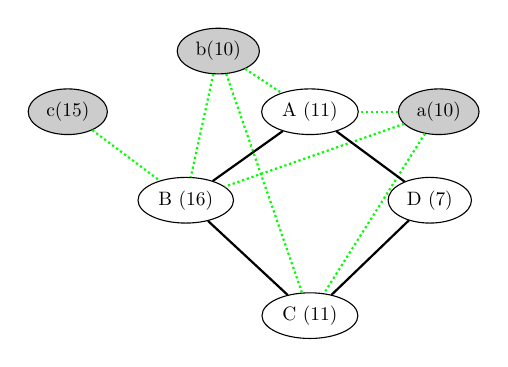
\begin{tikzpicture}
\usetikzlibrary{arrows}
\usetikzlibrary{shapes}
\tikzstyle{every node}=[draw, ellipse, minimum size=10pt,align=center,scale=0.7]
\node[fill=gray!40] at (0,0)(6){b(10)};
\node[below right=0.5cm of 6] (1){A (11)};
\node[below left=1cm of 1](2){B (16)};
\node[below right=1cm of 1](4){D (7)};
\node[below=2cm of 1](3){C (11)};
\node[fill=gray!40, right=0.5cm of 1] (5){a(10)};
\node[fill=gray!40, above left=1cm of 2] (7){c(15)};
\path[every node/.style={font=\sffamily\small},thick]
    (5) edge[green,densely dotted] node [] {} (1)
	edge[green,densely dotted] node [] {} (2)
	edge[green,densely dotted] node [] {} (3)
    (6) edge[green,densely dotted] node [] {} (1)
	edge[green,densely dotted] node [] {} (2)
	edge[green,densely dotted] node [] {} (3)
    (7) edge[green,densely dotted] node [] {} (2)
    (1) edge node [] {} (4)
    (2) edge node [] {} (3)
	edge node [] {} (1)
    (4) edge node [] {} (3);
\end{tikzpicture}
  \caption{Auxiliary graph for the input instance of Figure~\ref{fig:input}.\label{fig:aux}}   
\end{figure}

Paths in the auxiliary graph yield a valid column to the RMP if they respect some constraints.
Suppose we have to find a path to map the virtual link $(u,v)$.
First, the path has to contain exactly two auxiliary edges, that are the ones with endpoints in $u$ and $v$. This is easily enforced by setting a cost~$\infty$ to all auxiliary edges that connect auxiliary nodes other than $u$ or $v$.
Second, a path in the auxiliary graph has to contain at least one substrate edge, 
and the node adjacent to the source has to differ from the node adjacent to the target node. 
If one of these two conditions are not satisfied it means that both auxiliary nodes are mapped to the same substrate node, which is a restriction of the problem.
Hence, Dijkstra's algorithm cannot be directly applied to solve the pricing problem. 
Figure~\ref{fig:subprob} shows an example of a pricing problem. 
Auxiliary nodes are filled with gray and auxiliary edges are dotted. %The edges have costs associated with them.

\begin{figure}[h]
  \centering
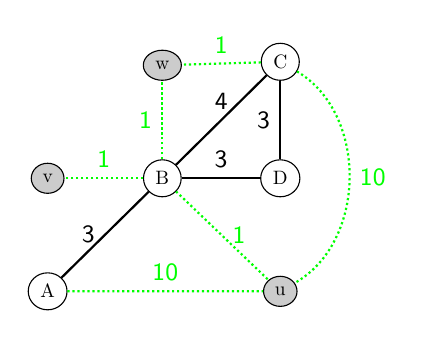
\begin{tikzpicture}
\usetikzlibrary{arrows}
\usetikzlibrary{shapes}
\tikzstyle{every node}=[draw, ellipse, minimum size=10pt,align=center,scale=0.7]
\node at (0,0)(B){B};
\node[right=1cm of B](D){D};
\node[fill=gray!40,left=1cm of B](v){v};
\node[below=1cm of v](A){A};
\node[above=1cm of D] (C){C};
\node[fill=gray!40,above=1cm of B] (w){w};
\node[fill=gray!40, below=1cm of D](u){u};
\path[every node/.style={font=\sffamily\small},thick]
    (A) edge[green,densely dotted] node [above] {10} (u)
    (B) edge node [left, above] {4} (C)
  edge[green,densely dotted] node [left] {1} (w)
	edge node [above] {3} (D)
	edge node [left] {3} (A)
	edge[green,densely dotted] node [right] {1} (u)
	edge[green,densely dotted] node [above] {1} (v)
    (C) edge node [left] {3} (D)
  edge[green,densely dotted] node [above] {1} (w)
  edge[green,densely dotted, bend left=60] node [right] {10} (u);
\end{tikzpicture}
  \caption{Subproblem graph\label{fig:subprob}}
\end{figure}


Suppose that we want to find a path between $u$ and~$v$ in the auxiliary graph.
The minimum-cost path in the graph $u - B - v$ does not contain any substrate edge and then is invalid.
The path $u - B - D - C - B - v$ is also invalid, because both~$u$ and $v$ are mapped to the same substrate node $B$.
The path $u - C - w - B - v$ is invalid because it uses auxiliary edges not connected to $u$ or $v$.
Therefore the minimum-cost valid path in the graph is $u - A - B - v$, where
node $u$ is mapped to $A$ and $v$ to $B$, and virtual link~$(u,v)$ is mapped to~$(A,B)$.
Note that the edge $(w,B)$ has a cost of $\infty$, so no path could use this auxiliary edge.

\subsection{Proposed Modified Dijkstra Algorithm}
We  propose a modified Dijkstra's algorithm (Algorithm~\ref{alg:dij}) to find a valid path with the minimum reduced cost.
It works as multiple Dijkstra's algorithms running in parallel.
Each node to be visited is associated with an origin, i.e. the first physical node in the path.
Initially all neighbors of the source node~$s$ are added to the priority queue $Q$, with an origin equal to itself.
At each iteration the node in the queue with the minimum distance is selected to be visited.
When the node~$v$ with origin~$w$ is visited, its neighbors are added to the queue with an origin~$w$ if it the cost of reaching the neighbor through $v$ is smaller than its current distance.
Hence the same node can be added multiple times if it is reached from different origins.
But the algorithm is still polynomial since the number of times each node will be visited is bound by the degree of~$s$.
The target~$t$ can only be added when the path contains at least one physical edge, this is detected by checking if the origin of the node is equal to itself.
The algorithm stops when the target node~$t$ is visited.

\begin{algorithm}
%\scriptsize
  \KwIn{Let $s$ be the source node, and $G^A = (V^A, E^A)$ be the auxiliary graph, and $c(u,v)$ the cost of the edge $(u,v)$.}
\KwOut{$d[v,w]$ is the cost of the minimum cost path from $s$ to $v$ with origin $w$.}
initialize every $d$ as $\infty$\;
\ForEach{edge $(s,v) \in E^{A}$}
{$d[v,v] := c(s,v)$\;
  $Q := Q \cup \{(v,v)\}$\;
}
\While{$Q$ is not empty}
  {$(u, origin) := extract\_min(Q)$\;
  \If{u = t}{return best path with cost $d[u,origin]$\;}
    \ForEach{edge $(u,v) \in E^{A}$}
    {\If{$v = t$ and $u = origin$}{continue\;}
      \If{$d[v,origin] < d[u, origin] + c(u,v)$}
      {$d[v, origin] := d[u, origin] + c(u,v)$\;
        \eIf{$(v,origin) \in Q$}
        {decrease cost of $(v,origin)$ in $Q$\;}
        {$Q := Q \cup \{(v,origin)\}$\;}
      }
    }
  }
\caption{Modified Dijkstra's Algorithm}
\label{alg:dij}
\end{algorithm}

\begin{proposition} The Modified Dijkstra's Algorithm finds a valid path to the problem with the smallest cost in the auxiliary graph in polynomial time.
\end{proposition}
\begin{proof}
  At each moment the set of nodes that were already visited have the shortest distance from the source node.
  A node is not visited more than its indegree, i.e., the number of arcs incoming that node.
  Suppose a node $u$ with cost $d$ that was already visited is adjacent to a node $v$ being visited with cost $d' < d$.
  This is an impossible situation because if $u$ has distance $d'<d$ it would be visited before $u$.
  So once a node is visited it has the smallest possible distance from the source.
  Thus once the target node $t$ is visited it has the smallest possible distance from the source.

  Moreover, the algorithm has to find the shortest distance taking into account the aforementioned constraints.
  With this aim, the target node $t$ can only be added to the queue if its predecessor is not equal to its origin.
  In that way the path obtained by this algorithm always contains at least one physical edge. Additionally, since there are no edges with negative costs, the path obtained does not contain a loop.
  This algorithm is polynomial and corresponds to run a Dijkstra algorithm for each node adjacent to the source node of $s$.
  Theoretically, this algorithm has a time complexity of $O(|E^S||V^S| + |V^S|^2log|V^S|)$ with Fibonacci heaps, and $O(|V^S||E^S|log|V^S|)$ with binary heaps.
\end{proof}

%Although there is a large number of paths, the column generation algorithm runs in polynomial time since the pricing problem is polynomial \cite{minoux:1986}.

%%%%%%%%%%%%%%%%%%%%%%%%%%%%%%%%%%%%%%%%%%%%%%%%%%%%%%%%
\section{Branch \& Price}
\label{sec:bp}

The column generation (CG) algorithm solves only the linear relaxation of the problem.
To obtain integer solutions for the VNEP, CG is embedded in a Branch \& Bound algorithm (B\&B).
A B\&B algorithm where each node is solved through a column generation is called Branch \& Price (B\&P).

We implemented a classic B\&P procedure which is summarized in Algorithm~\ref{alg:bp}.
Initially, the relaxation of the problem is solved.
If the optimal solution is not integral, the problem is split into two subproblems.
This process is called branching (Section~\ref{sec:branching}).
These subproblems are inserted in a priority queue with the key set to their relaxation value.
At each iteration, a subproblem is selected (Section~\ref{sec:nodesel}) from the queue and solved through a CG algorithm.
To speed up the algorithm by improving upper bounds, a constructive solution is build at each iteration (Section~\ref{sec:heur}) aiming to obtain an integral solution.
In case the incumbent integral solution has a better objective value than a subproblem relaxation, that branch is not expanded anymore since the relaxation of the problem is a lower bound on the integral solution.

\begin{algorithm}
$Q$ = {relaxation of IP}

\While{$Q$ is not empty}
  {
    subproblem = select\_node($Q$)\; \label{alg:genbp:snode}
    $x^*$ = solve subproblem using column generation\;
    \If{feasible($x^*$) and $\phi(x^*) < UB$}
    {\eIf{$x^*$ is integral}
      {$UB = \phi(x^*)$\;}
      {build heuristic solution\;
      split subproblem into subproblems and add them to $Q$\;\label{alg:bp:split}}
    }
  }
\caption{Branch \& Price Algorithm}
\label{alg:bp}
\end{algorithm}

The problems are branched with the introduction of cuts. Those cuts can turn the problem infeasible. 
New columns have to be inserted in order to make the problem feasible again.
The two-phase approach explained in Section~\ref{sec:cg} is used to overcome this problem.

Next we describe decisions taken by the B\&B for the VNEP we have implemented.

\subsection{Branching}
\label{sec:branching}
%A solution is fractional if one or more variables have a fractional value.
When expanding a node of the B\&B tree, if the solution is fractional, a variable is selected to be branched (Section~\ref{sec:varsel}).
The model solved at each node has two sets of decision variables: node mapping variables $x_{v,s}$ and path mapping variables $z_{p}$.
The former has a fixed size, while the latter grows during B\&P execution.
Therefore each one is treated differently. 

\subsubsection{Variable Selection}
\label{sec:varsel}
Variables $x_{v,s}$ are intregralized first starting with variable with values closest to $0.5$.
Once all variables $x$ are integral, path variables $z_{p}$ are verified in order of the origin node label.
Paths with the same origin are verified in the order they were generated. 

\subsubsection{Node mapping branching}
We tested two methods of branching for variables $x_{v,s}$.
In the first, two subproblems are created, one for which the substrate node $s$ is forbidden of hosting $v$ ($x_{v,s} \leq 0$) and another for which the node $s$ is forced to host $v$ ($v_{v,s} \geq 1$).
The second is called Generalized Upper Bound (GUB):
since $\sum\limits_{s' \in V^S} x_{v,s'} = 1$, one can cut more than one variable at a time. Two problems are created, one of which half the variables $x_{v}$ are forbidden by adding the cut $\sum\limits_{s < |V^S| / 2} x_{v,s} \leq 0$, and another for which the other half of variables are forbidden.
In both methods, the addition of cuts affect the pricing problem.
The auxiliary edge $(v,s)$ is either forbidden or fixed accordingly.

\subsubsection{Path branching}
Branching of path variables is not as straightforward as branching node variables. 
Individually branching on path variables would yield a large number of nodes to explore, since the number of paths grows exponentially with the size of the instance. 
To avoid this problem, paths are branched by introducing constraints that simulate restrictions on variables $y$ from the compact model. 
Suppose that for a given node, there exists one path variable $z_{p}$ that has a fractional value. Then there must be at least another variable $z_{p'}$ that is also fractional, since the sum of the variables that cover a virtual link is $1$. 
The paths $p$ and $p'$ associated to variables $z_{p}$ and $z_{p'}$ must have at least two different substrate edges $e \in p, e \notin p'$ and $f \in p', f \notin p$, otherwise they would be the same path. Then, two branches are generated, one with $e$ forbidden to belong to the path, and another for which $f$ is forbidden. Edges are not fixed, because it is easier to find a path that does not use multiple edges (it suffices to set their weights to a large value) than it is to fix edges. An edge $e$ is forbidden to be used to cover the virtual link $k$ by adding the cut $c(k,e) = \sum\limits_{p \in P^k} \delta_{e,p} z_p \leq 0$.

Adding these cuts affects the pricing problem. For each $k \in E^V$ and $e \in E^S$ a dual variable $\psi_{k,e}$ associated with the cut $c(k,e)$ is created. The values of these variables are added to the cost of each edge in the auxiliary graph. So each physical edge in the auxiliary graph has the cost $B_{k}(1 - y_{e} - \psi_{k,e})$.

\subsection{Node Selection}
\label{sec:nodesel}
The order in which active nodes are visited affects the performance of the algorithm. A balance has to be found between finding good upper bounds and visiting promising nodes. We tested three approaches: Depth First Search (DFS), Best First Search (BFS), and Best Projection (BPJ). DFS visits nodes in the order they are created. BFS visits first the most promising nodes, i.e., nodes with the lowest dual bound. BPJ visits nodes with fewer fractional variables first, since they are possibly closer to an integral solution.

\subsection{Heuristic Solution}
\label{sec:heur}
It was seen in Section~\ref{sec:prob}, that to obtain a feasible solution for the VNEP is NP-Hard.
Nevertheless, a greedy algorithm can be applied and in many situations is able to find a feasible solution.
Moreover, if part of the solution is already fixed, only the remaining part has to be constructed.
This happens when a greedy solution is applied on a subproblem, which uses all variables set on that branch of the B\&B tree since the root node.
Constructed feasible solutions can improve upper bounds allowing to prune entire branches of the B\&P search tree.

A solution obtained by the column generation may contain several fractional variables. 
The values of those variables contain valuable information about the problem. 
Each virtual node $v$ is mapped to the free physical node $s$ for which the value of $x_{v,s}$ is the largest. 
After all nodes are mapped, a breadth first search is used to map virtual links to paths in the physical substrate graph. The mapping of edges can fail if no path with enough bandwidth is found.

This algorithm is applied at each node of the B\&B tree. If a feasible solution is successfully built by the constructive heuristic algorithm, and the obtained solution is better than the current upper bound, the incumbent solution is updated.


%%%%%%%%%%%%%%%%%%%%%%%%%%%%%%%%%%%%%%%%%%%%%%%%%%%%%%%%
\section{Results}
\label{sec:results}
This section presents an experimental evaluation of the proposed B\&P algorithm. 
Results from B\&B are compared with results from the compact model presented in Section~\ref{sec:ILPmodel} solved with CPLEX\@. 
Three aspects of the algorithm are tested: the time spent to find the first integral solution, the running time, and the quality of solutions that were not proved to be optimal due to a time limit constraint. 
All tests were performed on a processor Intel Core i7 930 with 12 Gb of memory using a single thread. The commercial solver CPLEX 12.5 was used to solve the relaxed and integer models. All running times are in seconds, and a time limit of one hour was used in all runs.


\subsection{Datasets}

As virtualization is a fairly recent field, there is no established set of benchmark instances available for the VNEP\@.
The properties of physical substrate networks and virtual network embedding requests are not well understood~\cite{Chowdhury:2012}. Hence most works use synthetic networks \cite{FischerSurvey}.
Following this approach, all instances used in this experimental evaluation are generated with the GTI-ITM tool~\cite{Zagura:1996}.
This tool is capable of generating graphs with three different topologies: random, hierarchical and transit-stub.

Random instances are generated by spreading the nodes randomly in a 100 by 100 plane. These nodes are randomly linked using Waxman model \cite{Zagura:1996}. In this model, the probability of connecting two edges is $\alpha e^{- d / (100 \beta)}$, where $d$ is the Euclidean distance between the nodes, and $\alpha$ and $\beta$ are parameters. Thus, a larger $\alpha$ means a denser graph, and a larger $\beta$ means longer edges in the graph. Two types of random instances are generated: \textbf{Dense Random}, using $\alpha = 0.8$ and \textbf{Sparse Random}, using $\alpha = 0.5$. 
Both sets use $\beta = 0.2$.


\textbf{Hierarchical} instances are generated recursively. Initially, a random graph is created in a 100 by 100 plane. Then each node is replaced by a random graph with an average of five nodes. To generate those graphs the parameters $\alpha = 0.5$ and $\beta = 0.2$ were used.

\textbf{Transit-stub} is an hierarchical topology that best model the Internet~\cite{Zagura:1996}. Each node in a randomly generated graph is replaced by a subgraph called transit domain with an average of four nodes. To these domains are attached an average of three stub domains. Each stub domain has an average of two nodes. The transit domains as well as the stub domains are connected randomly with a probability $\alpha = 0.5$.

Each instance is composed of one physical substrate graph of one of the four topologies (Dense Random, Sparse Random, Hierarchical, Transit-stub) and one Sparse Random virtual network.  Only random virtual networks were generated because virtual networks tend to have a small number of nodes. Capacities of physical nodes and edges are randomly generated integers in the interval $[1,100]$. Considering the demands of virtual networks, two sets of instances were generated: one with \emph{low demand} with demands in the interval $[1,25]$, and another with \emph{high demand} with demands in the interval $[25,100]$.

As one of the purposes of this study is to test the limits of exact algorithms, large physical networks were generated.
Instances were generated from 20 to 200 nodes for random sparse and random dense topologies (6 sizes of substrate networks each).
For hierarchical instances, from 125 to 250 nodes (6 sizes of substrate networks). 
For Transit-stub, graphs from 90 to 270 nodes (5 sizes of substrate networks).
Virtual networks are in general small, and were generated from 2 to 18 nodes considering all even sizes in this interval.
Input data for the problem was build considering all combinations of substrate and virtual networks, and for each combination two instances are build considering a low and high demands of the substrate network.
Thus, in overall 414 instances were tested.


In Subsection~\ref{sec:param} we describe the parameter setting, while that in Section~\ref{sec:bptest} we present the B\&P results, and compare against the ones found by the compact model solved with CPLEX.

\subsection{Parameter Testing}
\label{sec:param}

As explained in the previous section, the node selection and branching methods influence the overall performance of the algorithm.
The following experiments compare different options for these components considering one instance for each size in a total of 414 instances.
The main metric used is the running time to obtain the optimal solution and the number of instances solved optimally in the available time limit.
Initially we tested the performance of the B\&B algorithm selecting nodes using  $DFS$, $BFS$, and $BPJ$ and results are summarized in Table~\ref{tab:nodesel}. 
The table shows for each of the four sets of instances, the number of tested instances in column \textbf{\#inst}, and for each node selection method, the number of optimal solutions found within the time limit in column~\textbf{\#opt}, and the average running time in seconds in column~\textbf{time(s)}.

\begin{table*}[h]
\begin{center}
  \caption{Node Selection Results}\label{tab:nodesel}
\begin{tabular} {l l | r r | r r | r r | r r }
\hline
                &                &  \multicolumn{2}{c|}{DFS}  & \multicolumn{2}{c|}{BFS}   & \multicolumn{2}{c|}{BPJ}  \\
  set           & \#inst           &  \#opt       & time(s)        & \#opt   & time(s)          & \#opt           & time(s)     & DFS $\sim$ BFS   & BPJ $\sim$ BFS  \\
 \hline 
 Random-Sparse  & 108            & 76         & 1086.20    & 85        & 851.90       & 83            & 863.66   & < $10^{-3}$         & 0.991          \\
 Random-Dense   & 108            & 78         & 961.50     & 88        & 792.10       & 87            & 691.44   & < $10^{-3}$         & 0.994          \\ 
 Hierarchical   & 108            & 62         & 1503.62    & 64        & 1375.61      & 59            & 1542.29  & < $10^{-3}$         & 0.035          \\
 Transit-stub   & 90             & 59         & 1393.76    & 66        & 1138.92      & 62            & 1294.34  & < $10^{-3}$         & 0.003          \\
\hline
\end{tabular}
\end{center}
\end{table*}

By comparing the number of optimal solutions and running time, $BFS$ is clearly the best method.
Using Wilcox Signed-rank test with a confidence interval of 95\%, our results show that $BFS$ has a better running time performance than $DFS$ for all instances.
With the same test, $BFS$ is significantly better for Hierarchical and Transit-stub instances.
Results for the Wilcox Signed-rank test performed are shown in Table~\ref{tab:nodesel}.

\begin{comment}
\begin{table*}[h]
\begin{center}
  \caption{Node Selection Results}\label{tab:wil}
\begin{tabular} {l l | r r | r r | r r | r r}
                &               &  \multicolumn{2}{c|}{DFS}  & \multicolumn{2}{c|}{BFS}   & \multicolumn{2}{c|}{BPJ} &               &                \\
  set           & size          &  optimal    & time        & optimal   & time          & \#opt       & time(s) 
 \hline 
 Random-Sparse  & 108            & 76         & 1086.198    & 85        & 851.900       & 83            & 863.664   & < $10^{-3}$         & 0.991         \\
 Random-Dense   & 108            & 78         & 961.499     & 88        & 792.101       & 87            & 691.442   & < $10^{-3}$         & 0.994         \\ 
 Hierarchical   & 108            & 62         & 1503.617    & 64        & 1375.611      & 59            & 1542.288  & < $10^{-3}$         & 0.035         \\
 Transit-stub   & 88             & 59         & 1393.760    & 66        & 1138.916      & 62            & 1294.336  & < $10^{-3}$         & 0.003         \\
\end{tabular}
\end{center}
\end{table*}
\end{comment}

Further tests were performed to compare normal branching of variables and GUB. 
Branching on variables is also significantly better than GUB with a confidence interval of 95\%.

\subsection{Branch \& Price Evaluation}
\label{sec:bptest}

  Results for the proposed B\&P algorithm with normal branching of variables and $BFS$ strategy for selecting nodes are presented in this section.
Moreover, we present results for the compact ILP Model from Section~\ref{sec:ILPmodel} for the sake of comparison.

%The two algorithms were run on the four sets of instances. 
For each instance size, three substrate networks and three virtual networks were randomly generated and combined to form nine different VNEP instances. The values in the results are the mean for the nine instances. In total 3726 instances compse the dataset.

All results are shown in Tables~\ref{tab:sparse}-\ref{tab:ts}. 
For summarizing results, each line corresponds to the mean values obtained by all instances run with the virtual network size $|V|$. 
We grouped instances in this fashion since time changes considerable with the size of virtual networks, and not much with the size of substrate networks.
Column \textbf{\#NF} is the mean number of instances that did not finish withing the time limit, i.e., 
either they did not prove solution optimality, or they did not prove solution infeasibility in less than an hour. 
Column \textbf{time\_int} shows the average time to obtain the first integer solution, when one was found. 
Columns \textbf{time(s)} and \textbf{cost} show the average running time and solution cost, respectively.

Figures~\ref{fig:timegraph}, \ref{fig:costgraph}, \ref{fig:optgraph}, and \ref{fig:fintgraph} demonstrate the behavior of the algorithms for all instances. All graphs compare the results for ILP solved with CPLEX in dashed lines, and B\&P with a solid line. 
Each figure contains four different graphs, one for each topology. 
Graphs show results for instances sorted alongside the x-axis first by the size of virtual nodes and second by the number of physical nodes. 
So for example the point corresponding to a random sparse instance with 4 virtual nodes and 20 physical nodes is right to left of the result of the instance with 4 virtual nodes and 40 physical substrate nodes. 
In that way it can be seen that the number of virtual nodes is a better predictor of the time complexity of each instance. 
Hence even instances with a large number of physical nodes can be easily solved by B\&P when there is at most 8 virtual nodes.

Figure~\ref{fig:timegraph} compares average running times. 
B\&P had a better running time for~80 of the~90 instance sizes of the Transit-stub set,~97 out of~108 for the hierarchical set, and for all but~3 and~4 instances for the dense and sparse sets, respectively.
Even though solving the large model is in general more expensive than solving the linear relaxation of the compact model, its better lower bounds and the better exploitation of the problem structure compensate for its longer running times.

Figure~\ref{fig:costgraph} shows the average cost obtained considering the best solution value of instances in which the algorithm was able to find at least one feasible solution within the time limit.
%Even though both algorithms are exact, a time limit was set for all tests. 
Those graphs show the cost of the best obtained solution on the time limit. 
These graphs show some discontinuities since in some cases algorithms were not able to find any feasible solution, or to prove infeasibility.

The number of instances solved can be seen in Figure~\ref{fig:optgraph}. It shows the number of instances out of 9 that were either proved optimal or infeasible. 

Figure~\ref{fig:fintgraph} shows the time to obtain the first integer solution. In those graphs it is clear that B\&P is able to find initial integer solutions quicker than CPLEX due to the constructive heuristic used in each node.

\begin{figure*}
        \centering
        \begin{subfigure}[b]{0.40\textwidth}
                \includegraphics[width=\textwidth]{graphs/time_fsparsevir4}
                \caption{Sparse Random}
                \label{fig:s11}
        \end{subfigure}
        ~ 
        \begin{subfigure}[b]{0.4\textwidth}
                \includegraphics[width=\textwidth]{graphs/time_fdensevir4}
                \caption{Dense Random}
                \label{fig:d11}
        \end{subfigure}
        \\
        \begin{subfigure}[b]{0.4\textwidth}
                \includegraphics[width=\textwidth]{graphs/time_fhiervir4}
                \caption{Hierarchical}
                \label{fig:h11}
        \end{subfigure}
        ~ 
        \begin{subfigure}[b]{0.4\textwidth}
                \includegraphics[width=\textwidth]{graphs/time_ftsvir4}
                \caption{Transit-stub}
                \label{fig:tstime}
        \end{subfigure}
        \caption{Average time in seconds.}\label{fig:timegraph}
\end{figure*}

\begin{figure*}
        \centering
        \begin{subfigure}[b]{0.40\textwidth}
                \includegraphics[width=\textwidth]{graphs/cost_fsparsevir4}
                \caption{Sparse Random}
                \label{fig:s12}
        \end{subfigure}
        ~
        \begin{subfigure}[b]{0.4\textwidth}
                \includegraphics[width=\textwidth]{graphs/cost_fdensevir4}
                \caption{Dense Random}
                \label{fig:d12}
        \end{subfigure}
        \\ 
        \begin{subfigure}[b]{0.4\textwidth}
                \includegraphics[width=\textwidth]{graphs/cost_fhiervir4}
                \caption{Hierarchical}
                \label{fig:h12}
        \end{subfigure}
        ~
        \begin{subfigure}[b]{0.4\textwidth}
                \includegraphics[width=\textwidth]{graphs/cost_ftsvir4}
                \caption{Transit-stub}
                \label{fig:t12}
        \end{subfigure}
        \caption{Average cost of feasible solutions.}\label{fig:costgraph}
\end{figure*}


\begin{figure*}
        \centering
        \begin{subfigure}[b]{0.40\textwidth}
                \includegraphics[width=\textwidth]{graphs/opt_fsparsevir4}
                \caption{Sparse Random}
                \label{fig:s21}
        \end{subfigure}
        ~
        \begin{subfigure}[b]{0.4\textwidth}
                \includegraphics[width=\textwidth]{graphs/opt_fdensevir4}
                \caption{Dense Random}
                \label{fig:d21}
        \end{subfigure}
        \\
        \begin{subfigure}[b]{0.4\textwidth}
                \includegraphics[width=\textwidth]{graphs/opt_fhiervir4}
                \caption{Hierarchical}
                \label{fig:h21}
        \end{subfigure}
        ~ 
        \begin{subfigure}[b]{0.4\textwidth}
                \includegraphics[width=\textwidth]{graphs/opt_ftsvir4}
                \caption{Transit-stub}
                \label{fig:t21}
        \end{subfigure}
        \caption{Number of instances solved.}\label{fig:optgraph}
\end{figure*}

\begin{figure*}
        \centering
        \begin{subfigure}[b]{0.40\textwidth}
                \includegraphics[width=\textwidth]{graphs/fint_fsparsevir4}
                \caption{Sparse Random}
                \label{fig:s22}
        \end{subfigure}
        ~
        \begin{subfigure}[b]{0.4\textwidth}
                \includegraphics[width=\textwidth]{graphs/fint_fdensevir4}
                \caption{Dense Random}
                \label{fig:d22}
        \end{subfigure}
        \\
        \begin{subfigure}[b]{0.4\textwidth}
                \includegraphics[width=\textwidth]{graphs/fint_fhiervir4}
                \caption{Hierarchical}
                \label{fig:h22}
        \end{subfigure}
        ~ 
        \begin{subfigure}[b]{0.4\textwidth}
                \includegraphics[width=\textwidth]{graphs/fint_ftsvir4}
                \caption{Transit-stub}
                \label{fig:t22}
        \end{subfigure}
        \caption{Time to obtain the first integer solution.}\label{fig:fintgraph}
\end{figure*}
\begin{comment}
\begin{figure*}
        \centering
        \begin{subfigure}[b]{0.40\textwidth}
                \includegraphics[width=\textwidth]{graphs/time_fsparsevir4}
                \caption{Average Time}
                \label{fig:s11}
        \end{subfigure}%
        ~ 
        \begin{subfigure}[b]{0.40\textwidth}
                \includegraphics[width=\textwidth]{graphs/cost_fsparsevir4}
                \caption{Average Cost of Feasible Solutions}
                \label{fig:s12}
        \end{subfigure}
        \\ 
        \begin{subfigure}[b]{0.40\textwidth}
                \includegraphics[width=\textwidth]{graphs/opt_fsparsevir4}
                \caption{Number of instances solved}
                \label{fig:s21}
        \end{subfigure}
        ~
        \begin{subfigure}[b]{0.40\textwidth}
                \includegraphics[width=\textwidth]{graphs/fint_fsparsevir4}
                \caption{Time to obtain first integer solution}
                \label{fig:s22}
        \end{subfigure}
        \caption{Sparse Random Instances}\label{fig:sparsegraph}
\end{figure*}

\begin{figure*}
        \centering
        \begin{subfigure}[b]{0.4\textwidth}
                \includegraphics[width=\textwidth]{graphs/time_fdensevir4}
                \caption{Average Time}
                \label{fig:d11}
        \end{subfigure}%
        ~ 
        \begin{subfigure}[b]{0.4\textwidth}
                \includegraphics[width=\textwidth]{graphs/cost_fdensevir4}
                \caption{Average Cost of Feasible Solutions}
                \label{fig:d12}
        \end{subfigure}
        \\ 
        \begin{subfigure}[b]{0.4\textwidth}
                \includegraphics[width=\textwidth]{graphs/opt_fdensevir4}
                \caption{Number of instances solved}
                \label{fig:d21}
        \end{subfigure}
        ~
        \begin{subfigure}[b]{0.4\textwidth}
                \includegraphics[width=\textwidth]{graphs/fint_fdensevir4}
                \caption{Time to obtain first integer solution}
                \label{fig:d22}
        \end{subfigure}
        \caption{Dense Random Instances}\label{fig:densegraph}
\end{figure*}

\begin{figure*}
        \centering
        \begin{subfigure}[b]{0.4\textwidth}
                \includegraphics[width=\textwidth]{graphs/time_fhiervir4}
                \caption{Average Time}
                \label{fig:h11}
        \end{subfigure}%
        ~ 
        \begin{subfigure}[b]{0.4\textwidth}
                \includegraphics[width=\textwidth]{graphs/cost_fhiervir4}
                \caption{Average Cost of Feasible Solutions}
                \label{fig:h12}
        \end{subfigure}
        ~ 
        \begin{subfigure}[b]{0.4\textwidth}
                \includegraphics[width=\textwidth]{graphs/opt_fhiervir4}
                \caption{Number of instances solved }
                \label{fig:h21}
        \end{subfigure}
        ~ 
        \begin{subfigure}[b]{0.4\textwidth}
                \includegraphics[width=\textwidth]{graphs/fint_fhiervir4}
                \caption{Time to obtain first integer solution}
                \label{fig:h22}
        \end{subfigure}
        \caption{Hierarchical Instances}\label{fig:hiergraph}
\end{figure*}

\begin{figure*}
        \centering
        \begin{subfigure}[b]{0.4\textwidth}
                \includegraphics[width=\textwidth]{graphs/time_ftsvir4}
                \caption{Average Time}
                \label{fig:t11}
        \end{subfigure}%
        ~ 
        \begin{subfigure}[b]{0.4\textwidth}
                \includegraphics[width=\textwidth]{graphs/cost_ftsvir4}
                \caption{Average Cost of Feasible Solutions}
                \label{fig:t12}
        \end{subfigure}
        ~ 
        \begin{subfigure}[b]{0.4\textwidth}
                \includegraphics[width=\textwidth]{graphs/opt_ftsvir4}
                \caption{Number of instances solved}
                \label{fig:t21}
        \end{subfigure}
        ~ 
        \begin{subfigure}[b]{0.4\textwidth}
                \includegraphics[width=\textwidth]{graphs/fint_ftsvir4}
                \caption{Time to obtain first integer solutions}
                \label{fig:t22}
        \end{subfigure}
        \caption{Transit-stub Instances}\label{fig:tsgraph}
\end{figure*}
\end{comment}

\begin{table*}[h]
\begin{center}
\caption{Results for sparse random instances.}\label{tab:sparse}
\begin{tabular} {l | r r r r | r r r r | r r r r | r r r r }
\hline
      &  \multicolumn{8}{c|}{ \textbf{Low Demand} } & \multicolumn{8}{c}{ \textbf{High Demand}} \\
      &  \multicolumn{4}{c|}{Branch \& Price} & \multicolumn{4}{c|}{CPLEX}    &       \multicolumn{4}{c|}{Branch \& Price} & \multicolumn{4}{c}{CPLEX}               \\  
$|V|$ & \#NF &  time\_int    &  time(s)       &  cost          &  \#NF &  time\_int  &  time(s)       &  cost  & \#NF &  time\_int    &  time(s)       &  cost          &  \#NF &  time\_int  &  time(s)       &  cost \\
\hline      
2&   0.00  &   0.04    &   0.04     &   16.33  & 0.00 & 0.06 & 0.13 & 16.33         & 0.00  &   0.02    &   0.02     &   19.71   & 0.00 & 0.06 & 0.13 & 19.61         \\  
4&   0.00  &   0.15    &   0.41     &   25.04  & 0.00 & 1.27 & 41.57 & 25.04        & 0.00  &   0.09    &   0.26     &   58.59   & 0.00 & 1.12 & 17.54 & 59.45        \\
6&   0.00  &   0.41    &   1.57     &   62.89  & 3.00 & 14.94 & 1580.90 & 63.17     & 0.00  &   0.17    &   1.72     &   127.97  & 2.17 & 10.61 & 1210.49 & 137.92    \\
8&   0.00  &   0.63    &   8.10     &   76.72  & 6.50 & 123.32 & 2733.78 & 77.91    & 0.00  &   0.32    &   2.92     &   166.08  & 4.50 & 62.90 & 2031.45 & 170.51    \\
10&  0.00  &   0.96    &   248.21   &   123.45 & 7.50 & 362.98 & 3071.16 & 132.59   & 0.00  &   0.39    &   13.68    &   192.87  & 6.00 & 349.79 & 2473.09 & 219.81   \\
12&  0.00  &   3.56    &   104.93   &   126.24 & 7.83 & 713.39 & 3163.46 & 154.21   & 0.00  &   0.77    &   26.72    &   268.61  & 6.33 & 826.02 & 2596.43 & 374.19   \\
14&  0.33  &   3.02    &   419.72   &   148.67 & 7.67 & 1063.17 & 3123.54 & 175.57  & 2.33  &   2.89    &   1078.41  &   424.19  & 6.50 & 1062.09 & 2719.31 & 536.23  \\
16&  1.00  &   5.75    &   748.51   &   218.54 & 7.67 & 1152.81 & 3117.38 & 298.26  & 5.00  &   1.90    &   2233.38  &   578.16  & 6.83 & 1570.38 & 2852.49 & 788.15  \\
18&  2.00  &   79.56   &   1426.87  &   233.56 & 7.50 & 1378.41 & 3012.03 & 326.40  & 4.83  &   2.73    &   2093.14  &   612.40  & 7.33 & 1930.45 & 2963.74 & 973.25  \\ 
\hline
\end{tabular} 
\end{center}
\end{table*}

\begin{table*}[h]
\begin{center}
\caption{Results for dense random instances.}\label{tab:dense}
\begin{tabular} {l | r r r r | r r r r | r r r r | r r r r }
\hline
      &  \multicolumn{8}{c|}{ \textbf{Low Demand} } & \multicolumn{8}{c}{ \textbf{High Demand}} \\
      &  \multicolumn{4}{c|}{Branch \& Price} & \multicolumn{4}{c|}{CPLEX}    &       \multicolumn{4}{c|}{Branch \& Price} & \multicolumn{4}{c}{CPLEX}               \\  
$|V|$ & \#NF &  time\_int    &  time(s)       &  cost          &  \#NF &  time\_int  &  time(s)       &  cost  & \#NF &  time\_int    &  time(s)       &  cost          &  \#NF &  time\_int  &  time(s)       &  cost \\
\hline      
2&     0.00  &   0.07    &   0.07     &   16.33   & 0.00 & 0.07 & 0.14 & 16.33         &    0.00  &   0.03    &   0.03     &   19.67    & 0.00 & 0.06 & 0.14 & 19.82              \\  
4&     0.00  &   0.28    &   0.71     &   25.00   & 0.00 & 1.34 & 96.69 & 25.00        &    0.00  &   0.14    &   0.44     &   56.77    & 0.00 & 1.23 & 23.55 & 56.87             \\
6&     0.00  &   0.55    &   4.29     &   62.67   & 3.67 & 14.75 & 1790.96 & 63.06     &    0.00  &   0.30    &   1.67     &   133.21   & 2.33 & 9.44 & 1372.85 & 141.74       \\
8&     0.00  &   1.02    &   23.11    &   76.72   & 7.00 & 142.51 & 2872.77 & 77.50    &    0.00  &   0.49    &   4.23     &   161.82   & 5.17 & 54.82 & 2313.42 & 163.81       \\
10&    0.17  &   7.38    &   324.63   &   121.78  & 7.33 & 463.34 & 3064.37 & 127.93   &    0.00  &   0.69    &   32.46    &   196.67   & 6.33 & 429.71 & 2859.08 & 205.82     \\
12&    0.00  &   2.77    &   196.70   &   126.61  & 8.00 & 739.44 & 3293.93 & 143.25   &    0.00  &   1.53    &   42.59    &   278.96   & 7.33 & 850.40 & 3001.72 & 371.76    \\
14&    0.33  &   9.06    &   555.80   &   148.24  & 8.00 & 1096.43 & 3246.88 & 166.88  &    2.00  &   3.78    &   1179.80  &   425.62   & 7.33 & 1041.58 & 3006.72 & 552.10   \\
16&    0.83  &   8.56    &   784.21   &   215.59  & 7.83  & 1155.70 & 3292.66 & 253.93 &    4.17  &   75.62   &   2187.54  &   556.50   & 7.50 & 906.56 & 3005.92 & 709.45   \\
18&    2.17  &   16.56   &   1545.78  &   232.27  & 8.50 & 893.13 & 3400.04 & 292.07   &    4.00  &   3.81    &   1940.83  &   548.83   & 7.50 & 1650.41 & 3000.13 & 682.96   \\ 
\hline
\end{tabular} 
\end{center}
\end{table*}

\begin{table*}[h]
\begin{center}
\caption{Hierarchical Instances}\label{tab:hier}
\begin{tabular} {l | r r r r | r r r r | r r r r | r r r r }
\hline
      &  \multicolumn{8}{c|}{ \textbf{Low Demand} } & \multicolumn{8}{c}{ \textbf{High Demand}} \\
      &  \multicolumn{4}{c|}{Branch \& Price} & \multicolumn{4}{c|}{CPLEX}    &       \multicolumn{4}{c|}{Branch \& Price} & \multicolumn{4}{c}{CPLEX}               \\  
$|V|$ & \#NF &  time\_int    &  time(s)       &  cost          &  \#NF &  time\_int  &  time(s)       &  cost  & \#NF &  time\_int    &  time(s)       &  cost          &  \#NF &  time\_int  &  time(s)       &  cost \\
\hline      
2&   0.00  &   0.02    &   0.02     &   16.33   & 0.00 & 0.11 & 0.26 & 16.33                 &  0.00  &   0.01    &   0.01     &   19.67   & 0.00 & 0.11 & 0.25 & 19.67                  \\  
4&   0.00  &   0.04    &   0.23     &   25.00   & 0.00 & 3.78 & 30.41 & 25.00                &  0.00  &   0.06    &   0.25     &   56.33   & 0.00 & 3.08 & 15.72 & 56.33                 \\
6&   0.00  &   0.24    &   0.99     &   62.67   & 1.00 & 32.77 & 1149.86 & 62.67            &  0.00  &   0.37    &   0.53     &   130.67  & 0.50 & 34.73 & 567.71 & 164.50          \\
8&   0.00  &   0.46    &   3.00     &   76.67   & 8.17 & 249.94 & 3499.51 & 80.00           &  0.00  &   0.63    &   5.55     &   161.04  & 4.17 & 234.69 & 2321.97 & 164.91          \\
10&  1.50  &   3.66    &   862.07   &   123.98  & 9.00 & 770.83 & 3600.00 & 167.09      &  0.00  &   1.65    &   10.90    &   192.15  & 8.33 & 905.15 & 3393.83 & 270.13        \\
12&  0.00  &   2.96    &   19.99    &   126.00  & 9.00 & 1221.98 & 3600.00 & 214.18    &  0.00  &   12.63   &   26.88    &   268.85  & 8.33 & 1863.78 & 3393.66 & 614.59      \\
14&  1.67  &   15.72   &   848.57   &   159.77  & 8.67 & 1943.51 & 3600.00 & 276.11    &  4.33  &   238.64  &   2222.53  &   461.47  & 8.00 & 2048.64 & 3355.05 & 668.70     \\
16&  2.67  &   38.43   &   1355.29  &   293.24  & 8.00 & 2360.40 & 3600.00 & 442.60   &  8.00  &   759.42  &   3316.40  &   771.28  & 8.50 & 1162.94 & 3448.68 & 759.00     \\
18&  9.00  &   306.44  &   3600.00  &   466.53  & 8.67 & 3201.44 & 3600.00 & 573.00   &  7.83  &   167.09  &   3159.66  &   666.50  & 7.17 & 2148.84 & 3391.17 & 682.50     \\ 
\hline
\end{tabular} 
\end{center}
\end{table*}

\begin{table*}[h]
\begin{center}
\caption{Results for transit-stub instances.}\label{tab:ts}
\begin{tabular} {l | r r r r | r r r r | r r r r | r r r r }
\hline
      &  \multicolumn{8}{c|}{ \textbf{Low Demand} } & \multicolumn{8}{c}{ \textbf{High Demand}} \\
      &  \multicolumn{4}{c|}{Branch \& Price} & \multicolumn{4}{c|}{CPLEX}    &       \multicolumn{4}{c|}{Branch \& Price} & \multicolumn{4}{c}{CPLEX}               \\  
$|V|$ & \#NF &  time\_int    &  time(s)       &  cost          &  \#NF &  time\_int  &  time(s)       &  cost  & \#NF &  time\_int    &  time(s)       &  cost          &  \#NF &  time\_int  &  time(s)       &  cost \\
\hline      
2&      0.00  &   0.02    &   0.02     &   16.33     & 0.00 & 0.11 & 0.26 & 16.33                &   0.00  &   0.01    &   0.01     &   19.67    & 0.00 & 0.11 & 0.24 & 19.67                  \\  
4&      0.00  &   0.03    &   0.09     &   25.40     & 0.00 & 3.75 & 30.41 & 25.00               &   0.00  &   0.05    &   0.19     &   56.33     & 0.00 & 3.30 & 16.54 & 56.33                 \\
6&      0.00  &   0.18    &   0.75     &   62.67     & 0.20 & 38.56 & 951.26 & 62.67             &   0.00  &   0.19    &   0.36     &   130.67   & 0.40 & 40.81 & 445.63 & 162.17           \\
8&      0.00  &   0.32    &   1.39     &   76.67     & 8.20 & 253.12 & 3492.03 & 82.36          &   0.00  &   0.31    &   1.02     &   160.22   & 3.20 & 330.52 & 1894.55 & 164.71           \\
10&     0.20  &   2.48    &   186.44   &   121.33    & 9.00 & 845.33 & 3600.00 & 166.20       &   0.00  &   1.78    &   4.32     &   191.40   & 6.80 & 1001.89 & 2957.12 & 267.28        \\
12&     0.00  &   2.74    &   12.05    &   126.00    & 9.00 & 1355.77 & 3600.00 & 198.94     &   0.00  &   6.33    &   9.83     &   269.95    & 7.60 & 1553.02 & 3208.40 & 394.55      \\
14&     0.20  &   15.14   &   254.96   &   148.29    & 9.00 & 1774.96 & 3600.00 & 253.97    &   2.60  &   141.40  &   1167.82  &   392.19   & 6.60 & 1499.95 & 2861.61 & 561.64     \\
16&     1.00  &   35.08   &   659.29   &   213.44    & 9.00 & 1766.10 & 3600.00 & 390.89    &   4.80  &   520.68  &   2340.14  &   583.17   & 6.60 & 1936.91 & 3146.33 & 801.06     \\
18&     3.00  &   77.88   &   1787.34  &   237.07    & 9.00 & 2519.80 & 3600.00 & 413.33    &   5.20  &   558.37  &   2338.52  &   632.32   & 8.00 & 1163.51 & 3254.62 & 666.50     \\ 
\hline
\end{tabular} 
\end{center}
\end{table*}

B\&P runs in significantly less time than CPLEX for most instances.% for almost all instances. 
Than, it is able to solve larger instances than CPLEX. 
For some hierarchical instances CPLEX consume all memory space and was not able to successfully find any solution.

The difference in performance is specially noticeable for larger instances. 
For example, for a substrate graph with a dense random topology and composed of 200 nodes, CPLEX was only able to solve instances with up to 4 virtual nodes, while B\&P could solve all instances with up to 10 nodes optimally in less than 10 minutes on average. 
Moreover, it was able to solve some of the larger instances in less than an hour.

CPLEX has a better performance for sets of instances with high demands, which contain more infeasible instances.
However, both algorithms have a harder time proving infeasibility.
Hence further study ought to be made investigating methods to detect infeasibility with the Branch \& Price algorithm.

%%%%%%%%%%%%%%%%%%%%%%%%%%%%%%%%%%%%%%%%%%%%%%%%%%%%%%%%

\section{Conclusion}
\label{sec:conclusion}
This work presented a new Branch \& Price algorithm for the Single-Path Virtual Network Embedding Problem.
It characterized the complexity of this problem by showing that finding a feasible solution for the VNEP is NP-Hard.
The master and pricing problem of a column generation algorithm were described in details and an algorithm to solve the pricing problem was thoroughly presented.
Implementation details were presented with alternative algorithms for node selection and branching.
Different implementations of B\&P were tested and the best version was compared with a compact model solved with CPLEX.
Algorithms were extensively tested by using four different topologies of different sizes, each with two settings of demands.

{ \color{red}
Results have shown that B\&P has a better performance and is able to solve larger instances than the standard model solved with CPLEX.
The presented B\&P is able to find optimal solutions for most instances with virtual networks of up to $8$ nodes. 
For example, for dense random instances with high demands, B\&P is able to solve six of the nine instances of 14 virtual nodes and 200 physical nodes, while CPLEX is able to solve only one instance of this size.
B\&P can also find integer solutions faster than CPLEX when one exists.
Thus the presented algorithm can be used in practice for small instances, can obtain good solutions for large instances, and can be used to evaluate heuristic algorithms since it is able to solve large instances in a reasonable time.
}

By exploiting the problem structure, B\&P is able to obtain good heuristic solutions quickly.
Those integer solutions provide high quality upper bounds that can prune large portions of the search tree, improving running time and reducing memory usage.
However, there is still room for improvement in the B\&P implementation.
The algorithm can be extended to a Branch \& Price \& Cut by adapting cover inequalities presented in~\cite{Barnhart:2000} for the Multicommodity Flow Problem.
Such cuts could reduce the number of nodes to explore, improving both the performance of the algorithm and the size of instances that the algorithm is able to solve.
Additionally, an adaption of the model to map multiple virtual networks simultaneously could improve resource utilization or other metrics such as revenue.
To implement this, a possible approach is that of \cite{Guerzoni:2014} of mapping virtual networks arriving in a window of time and allowing partial solutions to these networks.

\section*{Acknowledgement}
This work is supported by CNPq (Brazilian National Research Council), research project 462425/2014-2

\bibliographystyle{IEEEtran}
\bibliography{VNE}
\begin{comment}

ATTENTION : THE DATA BELOW IS OUTDATED
--------------------------------------

The following data was gathered with the old variable selection criterion (closest to 0.5)

\clearpage
\appendix

\newpage
\section{Full Results}

\begin{table*}[h]
\begin{center}
\caption{Sparse Random Instance - Low demands}
\begin{tabular} {l l | r r r r | r r r r}
\hline
       &                                &  \multicolumn{4}{c|}{Branch \& Price}                                & \multicolumn{4}{c}{CPLEX}                 \\
 $|S|$ & $|V|$                          &  \#NF    &  time\_int    &  time(s)       &  cost          &  \#NF &  time\_int  &  time(s)       &  cost          \\ 
\hline                                                                                                                           
 20 & 2                                  &   0             & 0.00          &  0.00       &  16.33       &  0           &  0.01     &  0.01       &  16.33           \\ 
 20 & 4                                  &   0             & 0.01          &  0.02       &  25.22       &  0           &  0.06     &  0.29       &  25.22           \\ 
 20 & 6                                  &   0             & 0.02          &  0.13       &  65.67       &  0           &  0.20     &  1.99       &  65.67           \\ 
 20 & 8                                  &   0             & 0.04          &  0.82       &  83.78       &  0           &  0.43     &  9.42       &  83.78           \\ 
 20 & 10                                 &   0             & 0.11          &  6.13       &  140.78      &  1           &  3.94     &  565.91     &  140.78          \\ 
 20 & 12                                 &   0             & 0.42          &  32.24      &  142.00      &  2           &  6.06     &  980.77     &  142.33          \\ 
 20 & 14                                 &   0             & 2.70          &  197.09     &  176.33      &  1           &  16.83    &  741.24     &  177.11          \\ 
 20 & 16                                 &   3             & 69.37         &  1465.91    &  303.00      &  1           &  22.56    &  704.30     &  304.88          \\ 
 20 & 18                                 &   3             & 397.88        &  1200.07    &  298         &  0           &  67.416   &  72.19      &  290             \\ 
 40 & 2                                  &   0             & 0.01          &  0.01       &  16.33       &  0           &  0.02     &  0.04       &  16.33           \\ 
 40 & 4                                  &   0             & 0.01          &  0.06       &  25.00       &  0           &  0.20     &  0.70       &  25.00           \\ 
 40 & 6                                  &   0             & 0.02          &  0.39       &  62.67       &  0           &  0.85     &  15.87      &  62.67           \\ 
 40 & 8                                  &   0             & 0.05          &  1.47       &  76.67       &  3           &  2.37     &  1993.26    &  76.67           \\ 
 40 & 10                                 &   0             & 0.06          &  198.00     &  121.11      &  8           &  4.61     &  3461.04    &  122.78          \\ 
 40 & 12                                 &   0             & 0.20          &  78.63      &  126.00      &  9           &  6.79     &  3600.00    &  127.67          \\ 
 40 & 14                                 &   1             & 0.11          &  701.76     &  146.56      &  9           &  11.39    &  3600.00    &  153.44          \\ 
 40 & 16                                 &   4             & 0.16          &  1837.95    &  215.22      &  9           &  417.85   &  3600.00    &  227.56          \\ 
 40 & 18                                 &   1             & 0.18          &  1120.02    &  221.11      &  9           &  371.33   &  3600.00    &  283.89          \\ 
 80 & 2                                  &   0             & 0.01          &  0.01       &  16.33       &  0           &  0.03     &  0.07       &  16.33           \\ 
 80 & 4                                  &   0             & 0.04          &  0.39       &  25.00       &  0           &  0.57     &  4.69       &  25.00           \\ 
 80 & 6                                  &   0             & 0.09          &  4.20       &  62.67       &  0           &  4.97     &  288.35     &  62.67           \\ 
 80 & 8                                  &   0             & 0.12          &  11.64      &  76.67       &  9           &  15.43    &  3600.00    &  76.67           \\ 
 80 & 10                                 &   0             & 0.28          &  255.95     &  120.67      &  9           &  32.48    &  3600.00    &  126.22          \\ 
 80 & 12                                 &   1             & 0.60          &  442.74     &  126.56      &  9           &  91.15    &  3600.00    &  134.56          \\ 
 80 & 14                                 &   0             & 0.53          &  1015.49    &  146.00      &  9           &  920.69   &  3600.00    &  185.00          \\ 
 80 & 16                                 &   4             & 0.40          &  1990.83    &  212.11      &  9           &  1182.38  &  3600.00    &  304.22          \\ 
 80 & 18                                 &   4             & 2.53          &  2092.46    &  223.67      &  9           &  943.55   &  3600.00    &  309.50          \\ 
 120 & 2                                 &   0             & 0.03          &  0.03       &  16.33       &  0           &  0.05     &  0.12       &  16.33           \\ 
 120 & 4                                 &   0             & 0.12          &  1.97       &  25.00       &  0           &  1.19     &  16.48      &  25.00           \\ 
 120 & 6                                 &   0             & 0.21          &  27.30      &  62.67       &  0           &  9.85     &  1979.18    &  62.67           \\ 
 120 & 8                                 &   0             & 0.36          &  55.61      &  76.67       &  9           &  49.50    &  3600.00    &  76.67           \\ 
 120 & 10                                &   0             & 0.61          &  696.93     &  120.67      &  9           &  259.51   &  3600.00    &  127.33          \\ 
 120 & 12                                &   0             & 1.49          &  372.39     &  126.00      &  9           &  739.56   &  3600.00    &  141.56          \\ 
 120 & 14                                &   2             & 1.91          &  1735.27    &  148.33      &  9           &  784.18   &  3600.00    &  170.62          \\ 
 120 & 16                                &   2             & 3.10          &  1706.44    &  212.44      &  9           &  1553.34  &  3600.00    &  320.14          \\ 
 120 & 18                                &   2             & 4.27          &  2026.57    &  222.11      &  9           &  2180.70  &  3600.00    &  290.62          \\ 
 160 & 2                                 &   0             & 0.07          &  0.07       &  16.33       &  0           &  0.09     &  0.20       &  16.33           \\ 
 160 & 4                                 &   0             & 0.26          &  8.99       &  25.00       &  0           &  2.16     &  71.25      &  25.00           \\ 
 160 & 6                                 &   0             & 0.45          &  78.36      &  62.67       &  9           &  24.79    &  3600.00    &  62.67           \\ 
 160 & 8                                 &   0             & 0.79          &  191.68     &  76.67       &  9           &  116.07   &  3600.00    &  76.67           \\ 
 160 & 10                                &   1             & 1.39          &  1527.90    &  121.56      &  9           &  811.94   &  3600.00    &  134.56          \\ 
 160 & 12                                &   1             & 2.53          &  891.74     &  126.56      &  9           &  1431.75  &  3600.00    &  194.78          \\ 
 160 & 14                                &   1             & 3.04          &  1841.81    &  148.00      &  9           &  1655.31  &  3600.00    &  177.75          \\ 
 160 & 16                                &   5             & 5.17          &  2724.22    &  229.44      &  9           &  2587.91  &  3600.00    &  334.50          \\ 
 160 & 18                                &   6             & 27.26         &  3233.96    &  239.78      &  9           &  3329.04  &  3600.00    &  458             \\ 
 200 & 2                                 &   0             & 0.15          &  0.15       &  16.33       &  0           &  0.15     &  0.32       &  16.33           \\ 
 200 & 4                                 &   0             & 0.56          &  6.88       &  25.00       &  0           &  3.43     &  156.03     &  25.00           \\ 
 200 & 6                                 &   0             & 1.77          &  218.34     &  62.67       &  9           &  48.95    &  3600.00    &  62.67           \\ 
 200 & 8                                 &   0             & 4.53          &  556.39     &  76.67       &  9           &  556.12   &  3600.00    &  77.00           \\ 
 200 & 10                                &   2             & 3.55          &  2371.14    &  121.78      &  9           &  1065.41  &  3600.00    &  143.89          \\ 
 200 & 12                                &   3             & 5.79          &  2351.89    &  128.56      &  9           &  2005.06  &  3600.00    &  184.38          \\ 
 200 & 14                                &   7             & 6.91          &  3316.64    &  162.44      &  9           &  2990.62  &  3600.00    &  189.50          \\ 
 200 & 16                                &   8             & 12.35         &  3543.59    &  236.44      &  9           &  -        &  3600.00    &  -               \\ 
 200 & 18                                &   9             & 8.99          &  3600.00    &  272.44      &  9           &  -        &  3600.00    &  -               \\ 
\hline
\end{tabular}
\end{center}
\end{table*}

\begin{table*}[h]
\begin{center}
\caption{Sparse Random Instances - High Demands}
\begin{tabular} {l l | r r r r | r r r r}
\hline
       &                                 &  \multicolumn{4}{c|}{Branch \& Price}                                & \multicolumn{4}{c}{CPLEX}                 \\
 $|S|$ & $|V|$                           &  \#NF  & time\_int     &  time(s)      &  cost            &  \#NF   &  time\_int   &  time(s)       &  cost       \\ 
 \hline       
20 & 2                                  &   0             & 0.00          &  0.00       &  19.89       &  0            &  0.01    &  0.01       &  19.89            \\ 
20 & 4                                  &   0             & 0.01          &  0.01       &  74.11       &  0            &  0.05    &  0.23       &  74.11            \\ 
20 & 6                                  &   0             & 0.01          &  0.06       &  154.17      &  0            &  0.14    &  0.57       &  154.17           \\ 
20 & 8                                  &   0             & 0.02          &  0.11       &  224.50      &  0            &  0.52    &  0.75       &  224.50           \\ 
20 & 10                                 &   0             & 0.06          &  0.57       &  250.20      &  0            &  1.68    &  2.19       &  250.20           \\ 
20 & 12                                 &   0             & 0.38          &  1.88       &  298.50      &  0            &  2.86    &  1.56       &  298.50           \\ 
20 & 14                                 &   0             & 2.045         &  2.86       &  461         &  0            &  11.604  &  1.69       &  461              \\ 
20 & 16                                 &   0             & -             &  0.04       &  -           &  0            &  -       &  0.37       &  -                \\ 
20 & 18                                 &   0             & -             &  0.04       &  -           &  0            &  -       &  0.49       &  -                \\ 
40 & 2                                  &   0             & 0.01          &  0.01       &  19.67       &  0            &  0.01    &  0.03       &  19.67            \\ 
40 & 4                                  &   0             & 0.01          &  0.07       &  57.67       &  0            &  0.18    &  0.50       &  57.67            \\ 
40 & 6                                  &   0             & 0.01          &  7.06       &  153.67      &  0            &  0.58    &  45.72      &  153.67           \\ 
40 & 8                                  &   0             & 0.02          &  0.75       &  160.56      &  0            &  0.97    &  53.59      &  160.56           \\ 
40 & 10                                 &   0             & 0.04          &  12.66      &  203.22      &  0            &  5.18    &  436.33     &  203.22           \\ 
40 & 12                                 &   0             & 0.05          &  508.49     &  287.67      &  2            &  9.25    &  1177.05    &  289.67           \\ 
40 & 14                                 &   3             & 0.27          &  1245.66    &  453.00      &  3            &  34.96   &  1914.15    &  446.56           \\ 
40 & 16                                 &   5             & 0.42          &  2259.53    &  596.33      &  5            &  70.18   &  2714.59    &  620.44           \\ 
40 & 18                                 &   6             & 3.90          &  3123.82    &  680.22      &  8            &  87.59   &  3381.96    &  661.89           \\ 
80 & 2                                  &   0             & 0.01          &  0.01       &  19.67       &  0            &  0.03    &  0.08       &  19.67            \\ 
80 & 4                                  &   0             & 0.05          &  0.34       &  56.33       &  0            &  0.46    &  2.42       &  56.33            \\ 
80 & 6                                  &   0             & 0.05          &  124.12     &  134.22      &  0            &  2.91    &  98.17      &  134.22           \\ 
80 & 8                                  &   0             & 0.07          &  3.79       &  159.67      &  0            &  8.02    &  1334.36    &  159.67           \\ 
80 & 10                                 &   0             & 0.16          &  19.63      &  191.00      &  9            &  21.66   &  3600.00    &  194.22           \\ 
80 & 12                                 &   3             & 0.25          &  1393.46    &  280.78      &  9            &  28.56   &  3600.00    &  305.89           \\ 
80 & 14                                 &   3             & 0.28          &  1485.60    &  419.11      &  9            &  425.16  &  3600.00    &  594.22           \\ 
80 & 16                                 &   6             & 0.40          &  2840.44    &  566.11      &  9            &  1312.95 &  3600.00    &  944.44           \\ 
80 & 18                                 &   6             & 0.68          &  2537.17    &  609.67      &  9            &  1878.77 &  3600.00    &  1053.78          \\ 
120 & 2                                 &   0             & 0.02          &  0.02       &  19.67       &  0            &  0.05    &  0.12       &  19.67            \\ 
120 & 4                                 &   0             & 0.07          &  1.89       &  56.33       &  0            &  1.15    &  10.75      &  56.33            \\ 
120 & 6                                 &   0             & 0.13          &  141.60     &  130.67      &  0            &  7.55    &  596.01     &  130.67           \\ 
120 & 8                                 &   0             & 0.19          &  18.34      &  159.67      &  9            &  29.01   &  3600.00    &  159.67           \\ 
120 & 10                                &   0             & 0.33          &  118.74     &  191.00      &  9            &  79.92   &  3600.00    &  204.89           \\ 
120 & 12                                &   4             & 0.51          &  2124.60    &  278.00      &  9            &  1035.93 &  3600.00    &  356.67           \\ 
120 & 14                                &   3             & 0.64          &  1738.19    &  404.67      &  9            &  1616.20 &  3600.00    &  598.50           \\ 
120 & 16                                &   7             & 0.75          &  3014.10    &  578.11      &  9            &  1541.42 &  3600.00    &  932.57           \\ 
120 & 18                                &   6             & 1.59          &  2689.84    &  613.22      &  9            &  2838.64 &  3600.00    &  1475.67          \\ 
160 & 2                                 &   0             & 0.04          &  0.04       &  19.67       &  0            &  0.09    &  0.21       &  19.67            \\ 
160 & 4                                 &   0             & 0.17          &  6.49       &  56.33       &  0            &  1.99    &  28.45      &  56.33            \\ 
160 & 6                                 &   0             & 0.36          &  292.52     &  130.67      &  4            &  17.57   &  2922.97    &  130.67           \\ 
160 & 8                                 &   0             & 1.33          &  94.32      &  159.67      &  9            &  122.95  &  3600.00    &  159.67           \\ 
160 & 10                                &   0             & 1.60          &  242.19     &  191.00      &  9            &  716.96  &  3600.00    &  211.11           \\ 
160 & 12                                &   3             & 0.98          &  2180.04    &  277.11      &  9            &  1478.29 &  3600.00    &  443.50           \\ 
160 & 14                                &   3             & 2.18          &  1983.75    &  404.22      &  9            &  1535.28 &  3600.00    &  558.50           \\ 
160 & 16                                &   8             & 1.92          &  3371.85    &  587.89      &  9            &  1942.46 &  3600.00    &  698.80           \\ 
160 & 18                                &   7             & 3.78          &  3038.77    &  641.67      &  9            &  2916.82 &  3600.00    &  701.67           \\ 
200 & 2                                 &   0             & 0.07          &  0.07       &  19.09       &  0            &  0.16    &  0.35       &  19.09            \\ 
200 & 4                                 &   0             & 0.32          &  15.20      &  55.90       &  0            &  2.92    &  62.91      &  55.90            \\ 
200 & 6                                 &   0             & 0.63          &  392.74     &  124.10      &  9            &  34.91   &  3599.52    &  124.10           \\ 
200 & 8                                 &   0             & 0.87          &  147.57     &  159.00      &  9            &  215.92  &  3600.00    &  159.00           \\ 
200 & 10                                &   0             & 1.30          &  610.86     &  193.90      &  9            &  1273.32 &  3600.00    &  255.20           \\ 
200 & 12                                &   5             & 2.28          &  2664.41    &  282.90      &  9            &  2401.21 &  3600.00    &  550.90           \\ 
200 & 14                                &   5             & 4.64          &  2891.79    &  418.30      &  9            &  2749.34 &  3600.00    &  558.60           \\ 
200 & 16                                &   8             & 6.32          &  3520.17    &  600.33      &  9            &  2984.89 &  3600.00    &  744.50           \\ 
200 & 18                                &   8             & 5.12          &  3553.89    &  651.67      &  9            &  -       &  3600.00    &  -                \\ 
\hline
\end{tabular}
\end{center}
\end{table*}

\begin{table*}[h]
\begin{center}
\caption{Dense Random Instances - Low Demands}
\begin{tabular} {l l | r r r r | r r r r}
\hline
       &                                 &  \multicolumn{4}{c|}{Branch \& Price}                                & \multicolumn{4}{c}{CPLEX}                 \\
 $|S|$ & $|V|$                           &  \#NF  & time\_int     &  time(s)      &  cost            &  \#NF   &  time\_int   &  time(s)       &  cost       \\ 
 \hline                                                                                                                                                      
 20 & 2                                  &  0           &  0.01         &  0.01      &  16.33           &  0            &   0.01       & 0.02        &  16.33       \\ 
 20 & 4                                  &  0           &  0.01         &  0.02      &  25.00           &  0            &   0.06       & 0.31        &  25.00       \\ 
 20 & 6                                  &  0           &  0.01         &  0.17      &  65.00           &  0            &   0.21       & 1.71        &  65.00       \\ 
 20 & 8                                  &  0           &  0.01         &  0.79      &  81.67           &  0            &   0.32       & 55.90       &  81.67       \\ 
 20 & 10                                 &  0           &  0.03         &  5.04      &  130.56          &  0            &   0.74       & 565.44      &  130.56      \\ 
 20 & 12                                 &  0           &  0.04         &  44.13     &  141.00          &  3            &   2.08       & 1763.58     &  141.33      \\ 
 20 & 14                                 &  0           &  0.04         &  110.10    &  164.22          &  3            &   3.55       & 1481.26     &  166.11      \\ 
 20 & 16                                 &  2           &  0.11         &  1112.67   &  253.33          &  2            &   12.04      & 1755.99     &  253.22      \\ 
 20 & 18                                 &  2           &  0.26         &  1323.39   &  242.00          &  6            &   5.61       & 2400.26     &  258.50      \\ 
 40 & 2                                  &  0           &  0.01         &  0.01      &  16.33           &  0            &   0.03       & 0.05        &  16.33       \\ 
 40 & 4                                  &  0           &  0.02         &  0.06      &  25.00           &  0            &   0.18       & 0.90        &  25.00       \\ 
 40 & 6                                  &  0           &  0.03         &  0.41      &  62.67           &  0            &   0.90       & 21.43       &  62.67       \\ 
 40 & 8                                  &  0           &  0.11         &  1.81      &  76.67           &  6            &   2.36       & 2780.74     &  76.67       \\ 
 40 & 10                                 &  0           &  0.10         &  18.07     &  120.67          &  8            &   5.88       & 3420.77     &  121.78      \\ 
 40 & 12                                 &  0           &  0.10         &  109.11    &  126.00          &  9            &   6.79       & 3600.00     &  126.33      \\ 
 40 & 14                                 &  0           &  0.20         &  47.50     &  146.00          &  9            &   32.44      & 3600.00     &  151.33      \\ 
 40 & 16                                 &  2           &  0.21         &  1178.12   &  211.78          &  9            &   93.98      & 3600.00     &  229.56      \\ 
 40 & 18                                 &  0           &  0.33         &  675.74    &  219.33          &  9            &   307.87     & 3600.00     &  272.11      \\ 
 80 & 2                                  &  0           &  0.02         &  0.02      &  16.33           &  0            &   0.03       & 0.06        &  16.33       \\ 
 80 & 4                                  &  0           &  0.09         &  0.67      &  25.00           &  0            &   0.50       & 8.83        &  25.00       \\ 
 80 & 6                                  &  0           &  0.15         &  7.34      &  62.67           &  0            &   5.13       & 508.01      &  62.67       \\ 
 80 & 8                                  &  0           &  0.27         &  21.62     &  76.67           &  9            &   16.14      & 3600.00     &  76.67       \\ 
 80 & 10                                 &  0           &  0.53         &  238.55    &  120.67          &  9            &   33.05      & 3600.00     &  121.56      \\ 
 80 & 12                                 &  0           &  0.56         &  93.00     &  126.00          &  9            &   195.71     & 3600.00     &  130.78      \\ 
 80 & 14                                 &  0           &  3.03         &  208.06    &  146.00          &  9            &   769.71     & 3600.00     &  170.22      \\ 
 80 & 16                                 &  2           &  1.76         &  1115.46   &  210.22          &  9            &   832.80     & 3600.00     &  253.56      \\ 
 80 & 18                                 &  0           &  1.15         &  1110.37   &  219.33          &  9            &   1114.13    & 3600.00     &  309.67      \\ 
 120 & 2                                 &  0           &  0.06         &  0.06      &  16.33           &  0            &   0.06       & 0.13        &  16.33       \\ 
 120 & 4                                 &  0           &  0.26         &  2.31      &  25.00           &  0            &   1.19       & 61.13       &  25.00       \\ 
 120 & 6                                 &  0           &  0.66         &  30.42     &  62.67           &  4            &   12.72      & 3014.61     &  62.67       \\ 
 120 & 8                                 &  0           &  1.07         &  83.87     &  76.67           &  9            &   53.40      & 3600.00     &  76.67       \\ 
 120 & 10                                &  0           &  5.56         &  465.39    &  120.67          &  9            &   271.11     & 3600.00     &  124.67      \\ 
 120 & 12                                &  0           &  2.64         &  463.21    &  126.00          &  9            &   791.47     & 3600.00     &  129.78      \\ 
 120 & 14                                &  0           &  4.82         &  1429.16   &  146.00          &  9            &   759.32     & 3600.00     &  167.11      \\ 
 120 & 16                                &  2           &  4.88         &  1840.23   &  213.44          &  9            &   1994.69    & 3600.00     &  286.00      \\ 
 120 & 18                                &  1           &  4.20         &  1947.06   &  221.11          &  9            &   2144.90    & 3600.00     &  328.00      \\ 
 160 & 2                                 &  0           &  0.13         &  0.13      &  16.33           &  0            &   0.10       & 0.22        &  16.33       \\ 
 160 & 4                                 &  0           &  0.58         &  8.86      &  25.00           &  0            &   2.33       & 110.77      &  25.00       \\ 
 160 & 6                                 &  0           &  1.08         &  103.41    &  62.67           &  9            &   23.64      & 3600.00     &  62.67       \\ 
 160 & 8                                 &  0           &  2.30         &  300.78    &  76.67           &  9            &   213.32     & 3600.00     &  76.67       \\ 
 160 & 10                                &  1           &  5.17         &  1648.07   &  120.89          &  9            &   1001.60    & 3600.00     &  131.22      \\ 
 160 & 12                                &  0           &  4.13         &  1595.81   &  126.00          &  9            &   1489.38    & 3600.00     &  165.00      \\ 
 160 & 14                                &  5           &  15.68        &  2824.43   &  152.33          &  9            &   2050.57    & 3600.00     &  187.75      \\ 
 160 & 16                                &  5           &  14.08        &  3332.66   &  225.56          &  9            &   2844.99    & 3600.00     &  247.33      \\ 
 160 & 18                                &  7           &  11.54        &  3463.64   &  237.33          &  9            &   -          & 3600.00     &  -           \\ 
 200 & 2                                 &  0           &  0.23         &  0.23      &  16.33           &  0            &   0.17       & 0.35        &  16.33       \\ 
 200 & 4                                 &  0           &  1.02         &  13.08     &  25.00           &  0            &   3.76       & 398.17      &  25.00       \\ 
 200 & 6                                 &  0           &  2.25         &  323.10    &  62.67           &  9            &   45.90      & 3600.00     &  62.67       \\ 
 200 & 8                                 &  0           &  3.07         &  820.89    &  76.67           &  9            &   569.53     & 3600.00     &  76.67       \\ 
 200 & 10                                &  3           &  11.50        &  2139.78   &  122.00          &  9            &   1467.65    & 3600.00     &  137.78      \\ 
 200 & 12                                &  4           &  9.65         &  2740.72   &  133.11          &  9            &   1951.19    & 3600.00     &  166.25      \\ 
 200 & 14                                &  7           &  48.99        &  3483.86   &  168.11          &  9            &   2963.01    & 3600.00     &  158.75      \\ 
 200 & 16                                &  9           &  27.83        &  3600.00   &  253.00          &  9            &   -          & 3600.00     &  -           \\ 
 200 & 18                                &  9           &  114.26       &  3600.00   &  285.56          &  9            &   -          & 3600.00     &  -           \\
\hline
\end{tabular}
\end{center}
\end{table*}

\begin{table*}[h]
\begin{center}
\caption{Dense Random Instances - High Demands}
\begin{tabular} {l l | r r r r | r r r r}
\hline
       &                                 &  \multicolumn{4}{c|}{Branch \& Price}                                & \multicolumn{4}{c}{CPLEX}                 \\
 $|S|$ & $|V|$                           &  \#NF  & time\_int     &  time(s)      &  cost            &  \#NF   &  time\_int   &  time(s)       &  cost       \\ 
\hline                                                                                                                                               
20 & 2                                  &  0           &  0.00        &  0.00        & 19.67           &  0            &  0.01        & 0.02         & 19.67       \\ 
20 & 4                                  &  0           &  0.01        &  0.02        & 59.00           &  0            &  0.09        & 0.28         & 59.00       \\ 
20 & 6                                  &  0           &  0.02        &  0.23        & 184.11          &  0            &  0.13        & 0.99         & 184.11      \\ 
20 & 8                                  &  0           &  0.01        &  0.38        & 183.67          &  0            &  0.25        & 2.34         & 183.67      \\ 
20 & 10                                 &  0           &  0.03        &  2.38        & 252.00          &  0            &  1.11        & 6.26         & 252.00      \\ 
20 & 12                                 &  0           &  0.09        &  12.53       & 348.14          &  0            &  2.03        & 10.32        & 348.14      \\ 
20 & 14                                 &  1           &  17.49       &  506.43      & 581.00          &  0            &  13.07       & 40.35        & 573.00      \\ 
20 & 16                                 &  1           &  147.92      &  827.49      & 719.40          &  0            &  20.92       & 35.50        & 719.40      \\ 
20 & 18                                 &  0           &  -           &  0.10        & -               &  0            &  -           & 0.79         & -           \\ 
40 & 2                                  &  0           &  0.01        &  0.01        & 19.67           &  0            &  0.01        & 0.04         & 19.67       \\ 
40 & 4                                  &  0           &  0.01        &  0.11        & 56.33           &  0            &  0.21        & 0.61         & 56.33       \\ 
40 & 6                                  &  0           &  0.02        &  7.15        & 135.44          &  0            &  0.57        & 13.48        & 135.44      \\ 
40 & 8                                  &  0           &  0.03        &  1.59        & 159.67          &  1            &  1.21        & 508.28       & 159.67      \\ 
40 & 10                                 &  0           &  0.03        &  8.47        & 191.00          &  3            &  2.79        & 2748.24      & 191.00      \\ 
40 & 12                                 &  1           &  0.09        &  776.44      & 272.44          &  9            &  3.49        & 3600.00      & 287.00      \\ 
40 & 14                                 &  3           &  0.13        &  1301.14     & 418.89          &  9            &  16.68       & 3600.00      & 435.22      \\ 
40 & 16                                 &  6           &  0.26        &  2472.04     & 546.56          &  9            &  33.87       & 3600.00      & 603.78      \\ 
40 & 18                                 &  6           &  0.25        &  2440.22     & 599.44          &  9            &  93.90       & 3600.00      & 667.44      \\ 
80 & 2                                  &  0           &  0.01        &  0.01        & 19.67           &  0            &  0.03        & 0.07         & 19.67       \\ 
80 & 4                                  &  0           &  0.05        &  0.42        & 56.33           &  0            &  0.42        & 3.79         & 56.33       \\ 
80 & 6                                  &  0           &  0.09        &  8.74        & 130.67          &  0            &  3.01        & 193.01       & 130.67      \\ 
80 & 8                                  &  0           &  0.12        &  7.50        & 159.67          &  6            &  9.88        & 2818.23      & 159.67      \\ 
80 & 10                                 &  0           &  0.23        &  26.20       & 191.00          &  9            &  13.04       & 3600.00      & 191.00      \\ 
80 & 12                                 &  1           &  0.25        &  649.88      & 269.56          &  9            &  78.74       & 3600.00      & 280.78      \\ 
80 & 14                                 &  3           &  0.43        &  1516.65     & 387.00          &  9            &  752.22      & 3600.00      & 496.56      \\ 
80 & 16                                 &  5           &  0.68        &  2298.35     & 517.22          &  9            &  950.62      & 3600.00      & 703.67      \\ 
80 & 18                                 &  6           &  0.87        &  2458.66     & 523.33          &  9            &  2107.12     & 3600.00      & 837.38      \\ 
120 & 2                                 &  0           &  0.03        &  0.03        & 19.67           &  0            &  0.06        & 0.13         & 19.67       \\ 
120 & 4                                 &  0           &  0.12        &  1.97        & 56.33           &  0            &  1.08        & 13.03        & 56.33       \\ 
120 & 6                                 &  0           &  0.20        &  94.95       & 130.67          &  0            &  7.97        & 1135.29      & 130.67      \\ 
120 & 8                                 &  0           &  0.54        &  31.71       & 159.67          &  7            &  31.22       & 3351.69      & 159.67      \\ 
120 & 10                                &  0           &  0.74        &  86.37       & 191.00          &  9            &  87.64       & 3600.00      & 195.56      \\ 
120 & 12                                &  2           &  0.83        &  1221.87     & 269.56          &  9            &  930.39      & 3600.00      & 316.56      \\ 
120 & 14                                &  0           &  1.58        &  1190.82     & 377.00          &  9            &  1681.89     & 3600.00      & 547.56      \\ 
120 & 16                                &  3           &  1.34        &  2118.18     & 501.56          &  9            &  1731.38     & 3600.00      & 799.38      \\ 
120 & 18                                &  6           &  1.87        &  2781.59     & 532.22          &  9            &  987.24      & 3600.00      & 748         \\ 
160 & 2                                 &  0           &  0.06        &  0.06        & 19.67           &  0            &  0.10        & 0.23         & 19.67       \\ 
160 & 4                                 &  0           &  0.29        &  9.51        & 56.33           &  0            &  1.82        & 38.95        & 56.33       \\ 
160 & 6                                 &  0           &  0.63        &  162.56      & 130.67          &  6            &  17.34       & 3294.34      & 130.67      \\ 
160 & 8                                 &  0           &  0.92        &  118.15      & 159.67          &  9            &  70.71       & 3600.00      & 159.67      \\ 
160 & 10                                &  0           &  1.35        &  328.35      & 191.00          &  9            &  606.78      & 3600.00      & 198.22      \\ 
160 & 12                                &  2           &  1.92        &  1539.68     & 272.00          &  9            &  1373.49     & 3600.00      & 405.50      \\ 
160 & 14                                &  3           &  2.72        &  1949.36     & 388.78          &  9            &  1472.87     & 3600.00      & 551.00      \\ 
160 & 16                                &  6           &  3.50        &  2985.52     & 552.44          &  9            &  1796.00     & 3600.00      & 721.00      \\ 
160 & 18                                &  7           &  13.63       &  3128.94     & 554.44          &  9            &  3413.39     & 3600.00      & 479         \\ 
200 & 2                                 &  0           &  0.10        &  0.10        & 20.57           &  0            &  0.17        & 0.37         & 20.57       \\ 
200 & 4                                 &  0           &  0.52        &  19.08       & 56.88           &  0            &  3.74        & 84.64        & 56.88       \\ 
200 & 6                                 &  0           &  1.00        &  452.59      & 138.88          &  8            &  27.60       & 3600.00      & 138.88      \\ 
200 & 8                                 &  0           &  2.44        &  346.62      & 160.50          &  8            &  215.63      & 3600.00      & 160.50      \\ 
200 & 10                                &  0           &  2.38        &  736.39      & 187.38          &  8            &  1866.90     & 3600.00      & 207.12      \\ 
200 & 12                                &  3           &  3.98        &  2907.43     & 275.25          &  8            &  2714.27     & 3600.00      & 592.60      \\ 
200 & 14                                &  3           &  7.33        &  2398.76     & 432.62          &  8            &  2312.73     & 3600.00      & 709.25      \\ 
200 & 16                                &  9           &  15.42       &  3600.00     & 602.78          &  9            &  -           & 3600.00      & -           \\ 
200 & 18                                &  9           &  9.73        &  3600.00     & 625.33          &  9            &  -           & 3600.00      & -           \\
\hline
\end{tabular}
\end{center}
\end{table*}

\begin{table*}
\begin{center}
\caption{Hierarchical Instances - Low Demands}
\begin{tabular} {l l | r r r r | r r r r}
\hline
       &                                 &  \multicolumn{4}{c|}{Branch \& Price}                                & \multicolumn{4}{c}{CPLEX}                 \\
 $|S|$ & $|V|$                           &  \#NF  & time\_int     &  time(s)      &  cost            &  \#NF   &  time\_int   &  time(s)       &  cost       \\ 
\hline
125 & 2   &  0            &  0.01          &  0.01        &  16.33     &  0           &  0.06            &  0.13       &  16.33     \\ 
125 & 4   &  0            &  0.11          &  0.29        &  25.00     &  0           &  2.27            &  9.18       &  25.00     \\ 
125 & 6   &  0            &  0.36          &  4.87        &  62.67     &  0           &  17.30           &  167.21     &  62.67     \\ 
125 & 8   &  0            &  1.15          &  29.32       &  76.67     &  5           &  75.18           &  3056.65    &  78.22     \\ 
125 & 10  &  4            &  13.63         &  1929.54     &  135.22    &  9           &  270.71          &  3600.00    &  151.78    \\ 
125 & 12  &  3            &  65.85         &  1389.12     &  144.89    &  9           &  629.59          &  3600.00    &  169.33    \\ 
125 & 14  &  9            &  182.92        &  3600.00     &  264.00    &  9           &  1538.64         &  3600.00    &  217.00    \\ 
125 & 16  &  9            &  857.62        &  3600.00     &  488.50    &  9           &  3142.99         &  3600.00    &  406.33    \\ 
125 & 18  &  9            &  916.42        &  3600.00     &  601.33    &  9           &  -               &  3600.00    &  -         \\ 
150 & 2   &  0            &  0.01          &  0.01        &  16.33     &  0           &  0.06            &  0.15       &  16.33     \\ 
150 & 4   &  0            &  0.03          &  0.28        &  25.00     &  0           &  2.06            &  10.77      &  25.00     \\ 
150 & 6   &  0            &  0.35          &  6.15        &  62.67     &  0           &  13.70           &  260.67     &  62.67     \\ 
150 & 8   &  0            &  0.64          &  33.88       &  76.67     &  8           &  68.72           &  3540.39    &  77.11     \\ 
150 & 10  &  4            &  2.25          &  1888.93     &  131.89    &  9           &  218.09          &  3600.00    &  155.33    \\ 
150 & 12  &  4            &  2.95          &  1998.31     &  135.44    &  9           &  922.26          &  3600.00    &  185.56    \\ 
150 & 14  &  7            &  12.57         &  2961.95     &  215.89    &  9           &  951.29          &  3600.00    &  263.50    \\ 
150 & 16  &  9            &  26.20         &  3600.00     &  410.33    &  9           &  855.97          &  3600.00    &  419.33    \\ 
150 & 18  &  9            &  155.34        &  3600.00     &  448.11    &  9           &  -               &  3600.00    &  -         \\ 
175 & 2   &  0            &  0.01          &  0.01        &  16.33     &  0           &  0.09            &  0.20       &  16.33     \\ 
175 & 4   &  0            &  0.03          &  0.84        &  25.00     &  0           &  2.57            &  19.25      &  25.00     \\ 
175 & 6   &  0            &  0.05          &  6.64        &  62.67     &  0           &  22.57           &  646.73     &  62.67     \\ 
175 & 8   &  0            &  0.36          &  32.48       &  76.67     &  9           &  108.28          &  3600.00    &  77.67     \\ 
175 & 10  &  4            &  2.23          &  1782.50     &  128.78    &  9           &  519.80          &  3600.00    &  166.00    \\ 
175 & 12  &  4            &  5.99          &  1722.29     &  136.89    &  9           &  873.28          &  3600.00    &  233.33    \\ 
175 & 14  &  7            &  13.50         &  2826.14     &  201.44    &  9           &  1429.26         &  3600.00    &  305.78    \\ 
175 & 16  &  9            &  25.24         &  3600.00     &  335.00    &  8           &  2425.69         &  3600.00    &  514.00    \\ 
175 & 18  &  9            &  19.76         &  3600.00     &  439.67    &  8           &  3201.44         &  3600.00    &  573.00    \\ 
200 & 2   &  0            &  0.01          &  0.01        &  16.33     &  0           &  0.11            &  0.25       &  16.33     \\ 
200 & 4   &  0            &  0.03          &  2.18        &  25.00     &  0           &  3.87            &  31.70      &  25.00     \\ 
200 & 6   &  0            &  0.06          &  19.37       &  62.67     &  1           &  28.18           &  1236.67    &  62.67     \\ 
200 & 8   &  0            &  0.25          &  83.65       &  76.67     &  9           &  161.43          &  3600.00    &  79.00     \\ 
200 & 10  &  4            &  2.69          &  2088.51     &  128.44    &  9           &  1038.06         &  3600.00    &  166.22    \\ 
200 & 12  &  2            &  3.44          &  1461.63     &  132.67    &  9           &  1293.03         &  3600.00    &  212.88    \\ 
200 & 14  &  6            &  19.43         &  2565.80     &  199.89    &  7           &  1875.52         &  3600.00    &  283.33    \\ 
200 & 16  &  9            &  26.12         &  3600.00     &  394.11    &  7           &  3016.97         &  3600.00    &  430.75    \\ 
200 & 18  &  9            &  28.82         &  3600.00     &  595.67    &  8           &  -               &  3600.00    &  -         \\ 
225 & 2   &  0            &  0.02          &  0.02        &  16.33     &  0           &  0.19            &  0.43       &  16.33     \\ 
225 & 4   &  0            &  0.04          &  1.26        &  25.00     &  0           &  5.72            &  47.53      &  25.00     \\ 
225 & 6   &  0            &  0.82          &  15.46       &  62.67     &  1           &  56.71           &  1890.65    &  62.67     \\ 
225 & 8   &  0            &  0.47          &  71.10       &  76.67     &  9           &  499.16          &  3600.00    &  86.22     \\ 
225 & 10  &  6            &  1.63          &  2466.65     &  136.00    &  9           &  1434.67         &  3600.00    &  180.00    \\ 
225 & 12  &  5            &  9.57          &  2070.26     &  144.44    &  9           &  1578.52         &  3600.00    &  273.33    \\ 
225 & 14  &  6            &  13.49         &  2598.64     &  228.11    &  9           &  2677.50         &  3600.00    &  291.29    \\ 
225 & 16  &  9            &  33.93         &  3600.00     &  369.00    &  9           &  -               &  3600.00    &  -         \\ 
225 & 18  &  9            &  53.11         &  3600.00     &  603.78    &  -           &  -               &  -          &  -         \\ 
250 & 2   &  0            &  0.02          &  0.02        &  16.33     &  0           &  0.18            &  0.41       &  16.33     \\ 
250 & 4   &  0            &  0.05          &  0.82        &  25.00     &  0           &  6.17            &  64.05      &  25.00     \\ 
250 & 6   &  0            &  0.31          &  22.09       &  62.67     &  4           &  58.16           &  2697.23    &  62.67     \\ 
250 & 8   &  0            &  1.18          &  143.34      &  76.67     &  9           &  586.85          &  3600.00    &  81.78     \\ 
250 & 10  &  4            &  5.73          &  2781.41     &  130.44    &  9           &  1143.66         &  3600.00    &  183.22    \\ 
250 & 12  &  3            &  3.96          &  1632.76     &  133.89    &  9           &  2035.18         &  3600.00    &  210.67    \\ 
250 & 14  &  8            &  19.96         &  3228.64     &  196.89    &  9           &  3188.84         &  3600.00    &  295.75    \\ 
250 & 16  &  9            &  16.32         &  3600.00     &  349.44    &  6           &  -               &  3600.00    &  -         \\ 
250 & 18  &  9            &  6.83          &  3600.00     &  507.89    &  -           &  -               &  -          &  -         \\
\hline
\end{tabular}
\end{center}
\end{table*}


\begin{table*}[h]
\begin{center}
\caption{Hierarchical Instances - High Demands}
\begin{tabular} {l l | r r r r | r r r r}
\hline
       &                                 &  \multicolumn{4}{c|}{Branch \& Price}                                & \multicolumn{4}{c}{CPLEX}                 \\
 $|S|$ & $|V|$                           &  \#NF  & time\_int     &  time(s)      &  cost            &  \#NF   &  time\_int   &  time(s)       &  cost       \\ 
\hline
125 & 2   &  0            &  0.01          &  0.01        &  19.67     &  0           &  0.05            &  0.11       &  19.67     \\ 
125 & 4   &  0            &  0.05          &  0.22        &  56.33     &  0           &  1.72            &  4.52       &  56.33     \\ 
125 & 6   &  1            &  70.59         &  439.99      &  180.89    &  0           &  17.85           &  58.07      &  180.89    \\ 
125 & 8   &  0            &  1.08          &  9.08        &  164.67    &  0           &  50.23           &  458.09     &  164.67    \\ 
125 & 10  &  1            &  8.93          &  799.98      &  229.67    &  6           &  204.63          &  2701.86    &  237.33    \\ 
125 & 12  &  9            &  57.62         &  3600.00     &  369.29    &  7           &  629.25          &  2889.93    &  389.00    \\ 
125 & 14  &  4            &  350.70        &  1866.99     &  499.67    &  4           &  636.09          &  2227.06    &  445.83    \\ 
125 & 16  &  7            &  1560.21       &  2827.93     &  672.33    &  6           &  1214.45         &  2692.10    &  726.00    \\ 
125 & 18  &  7            &  126.055       &  2801.42     &  783       &  6           &  1549.83         &  2774.42    &  569.00    \\ 
150 & 2   &  0            &  0.01          &  0.01        &  19.67     &  0           &  0.06            &  0.15       &  19.67     \\ 
150 & 4   &  0            &  0.04          &  0.41        &  56.33     &  0           &  2.28            &  6.84       &  56.33     \\ 
150 & 6   &  2            &  4.23          &  830.02      &  161.88    &  0           &  19.39           &  77.69      &  161.88    \\ 
150 & 8   &  0            &  1.09          &  26.19       &  171.11    &  0           &  70.36           &  1479.70    &  171.11    \\ 
150 & 10  &  1            &  2.58          &  1007.59     &  240.89    &  8           &  409.67          &  3261.10    &  266.33    \\ 
150 & 12  &  9            &  76.04         &  3600.00     &  438.50    &  7           &  597.23          &  3072.05    &  468.75    \\ 
150 & 14  &  7            &  197.97        &  3032.94     &  473.17    &  8           &  1262.33         &  3503.23    &  591.17    \\ 
150 & 16  &  9            &  287.46        &  3600.00     &  660.67    &  9           &  1111.43         &  3600.00    &  792.00    \\ 
150 & 18  &  7            &  129.69        &  2854.57     &  659.67    &  8           &  2747.84         &  3381.41    &  796       \\ 
175 & 2   &  0            &  0.01          &  0.01        &  19.67     &  0           &  0.09            &  0.20       &  19.67     \\ 
175 & 4   &  0            &  0.08          &  0.65        &  56.33     &  0           &  2.40            &  10.69      &  56.33     \\ 
175 & 6   &  2            &  3.03          &  819.05      &  170.00    &  1           &  22.56           &  703.68     &  167.00    \\ 
175 & 8   &  0            &  0.81          &  19.08       &  159.67    &  5           &  119.17          &  2675.24    &  161.22    \\ 
175 & 10  &  1            &  2.42          &  868.06      &  202.78    &  9           &  509.45          &  3600.00    &  259.44    \\ 
175 & 12  &  9            &  18.90         &  3600.00     &  425.00    &  9           &  1813.97         &  3600.00    &  493.17    \\ 
175 & 14  &  7            &  57.18         &  3181.59     &  396.67    &  9           &  2819.76         &  3600.00    &  806.50    \\ 
175 & 16  &  9            &  287.10        &  3600.00     &  986.75    &  9           &  -               &  3600.00    &  -         \\ 
175 & 18  &  9            &  70.71         &  3600.00     &  954.75    &  9           &  -               &  3600.00    &  -         \\ 
200 & 2   &  0            &  0.01          &  0.01        &  19.67     &  0           &  0.11            &  0.26       &  19.67     \\ 
200 & 4   &  0            &  0.04          &  1.67        &  56.33     &  0           &  3.25            &  15.48      &  56.33     \\ 
200 & 6   &  3            &  6.99          &  1205.31     &  149.38    &  1           &  17.34           &  659.21     &  148.25    \\ 
200 & 8   &  0            &  3.33          &  38.29       &  162.56    &  6           &  197.57          &  2769.50    &  162.56    \\ 
200 & 10  &  1            &  5.22          &  1554.55     &  204.33    &  9           &  821.48          &  3600.00    &  277.56    \\ 
200 & 12  &  9            &  126.25        &  3600.00     &  360.62    &  9           &  2250.90         &  3600.00    &  554.86    \\ 
200 & 14  &  8            &  103.62        &  3342.64     &  398.33    &  9           &  2324.11         &  3600.00    &  634       \\ 
200 & 16  &  9            &  188.44        &  3600.00     &  578.50    &  9           &  -               &  3600.00    &  -         \\ 
200 & 18  &  8            &  865.91        &  3218.07     &  1042.25   &  9           &  -               &  3600.00    &  -         \\ 
225 & 2   &  0            &  0.01          &  0.01        &  19.67     &  0           &  0.15            &  0.34       &  19.67     \\ 
225 & 4   &  0            &  0.15          &  1.40        &  56.33     &  0           &  3.52            &  23.51      &  56.33     \\ 
225 & 6   &  3            &  3.18          &  1212.33     &  163.11    &  0           &  69.38           &  697.81     &  159.11    \\ 
225 & 8   &  0            &  1.64          &  81.44       &  160.44    &  7           &  359.11          &  3273.55    &  162.56    \\ 
225 & 10  &  4            &  2.54          &  2080.56     &  222.33    &  9           &  1689.94         &  3600.00    &  284.44    \\ 
225 & 12  &  9            &  13.98         &  3600.00     &  439.78    &  9           &  2448.91         &  3600.00    &  951.75    \\ 
225 & 14  &  9            &  79.15         &  3600.00     &  459.00    &  9           &  -               &  3600.00    &  -         \\ 
225 & 16  &  9            &  333.86        &  3600.00     &  737.67    &  9           &  -               &  3600.00    &  -         \\ 
225 & 18  &  9            &  39.84         &  3600.00     &  598.67    &  2           &  -               &  3600.00    &  -         \\ 
250 & 2   &  0            &  0.01          &  0.01        &  19.67     &  0           &  0.19            &  0.42       &  19.67     \\ 
250 & 4   &  0            &  0.09          &  1.58        &  56.33     &  0           &  5.34            &  33.30      &  56.33     \\ 
250 & 6   &  3            &  1.80          &  1207.01     &  176.89    &  1           &  61.85           &  1209.78    &  169.89    \\ 
250 & 8   &  0            &  0.77          &  42.30       &  160.11    &  7           &  611.69          &  3275.76    &  167.33    \\ 
250 & 10  &  5            &  4.44          &  2128.35     &  205.11    &  9           &  1795.74         &  3600.00    &  295.71    \\ 
250 & 12  &  9            &  96.17         &  3600.00     &  400.22    &  9           &  3442.45         &  3600.00    &  830.00    \\ 
250 & 14  &  9            &  372.61        &  3600.00     &  775.25    &  9           &  3200.92         &  3600.00    &  866       \\ 
250 & 16  &  9            &  514.31        &  3600.00     &  1275.00   &  9           &  -               &  3600.00    &  -         \\ 
250 & 18  &  9            &  111.09        &  3600.00     &  940.80    &  -           &  -               &  -          &  -         \\ 
\hline
\end{tabular}
\end{center}
\end{table*}


\begin{table*}[h]
\begin{center}
\caption{Transit-Stub Instances - Low Demands}
\begin{tabular} {l l | r r r r | r r r r}
\hline
       &                                 &  \multicolumn{4}{c|}{Branch \& Price}                                & \multicolumn{4}{c}{CPLEX}                 \\
 $|S|$ & $|V|$                           &  \#NF  & time\_int     &  time(s)      &  cost            &  \#NF   &  time\_int   &  time(s)       &  cost       \\ 
\hline
90 & 2                              &  0                 &  0.01          &  0.01       &  16.33       &  0          &  0.04            &  0.08       &  16.33     \\ 
90 & 4                              &  0                 &  0.02          &  0.10       &  25.00       &  0          &  1.43            &  3.92       &  25.00     \\ 
90 & 6                              &  0                 &  0.15          &  1.10       &  62.67       &  0          &  6.16            &  80.43      &  62.67     \\ 
90 & 8                              &  0                 &  0.71          &  11.62      &  76.67       &  5          &  14.09           &  3060.16    &  76.67     \\ 
90 & 10                             &  0                 &  0.90          &  562.50     &  126.11      &  9          &  56.14           &  3600.00    &  135.44    \\ 
90 & 12                             &  4                 &  0.90          &  1936.71    &  137.44      &  9          &  420.97          &  3600.00    &  158.44    \\ 
90 & 14                             &  6                 &  4.25          &  2529.66    &  168.89      &  9          &  1295.66         &  3600.00    &  242.62    \\ 
90 & 16                             &  9                 &  7.64          &  3600.00    &  261.00      &  9          &  1668.90         &  3600.00    &  347.17    \\ 
90 & 18                             &  8                 &  54.70         &  3545.14    &  277.00      &  9          &  1630.65         &  3600.00    &  381.50    \\ 
135 & 2                             &  0                 &  0.01          &  0.01       &  16.33       &  0          &  0.05            &  0.12       &  16.33     \\ 
135 & 4                             &  0                 &  0.03          &  0.37       &  25.00       &  0          &  1.88            &  8.17       &  25.00     \\ 
135 & 6                             &  0                 &  0.73          &  4.26       &  62.67       &  0          &  16.24           &  207.81     &  62.67     \\ 
135 & 8                             &  0                 &  0.95          &  15.40      &  76.67       &  9          &  24.20           &  3600.00    &  78.11     \\ 
135 & 10                            &  1                 &  4.86          &  1008.53    &  125.56      &  9          &  119.30          &  3600.00    &  145.11    \\ 
135 & 12                            &  4                 &  11.38         &  1698.08    &  136.11      &  9          &  1072.44         &  3600.00    &  179.25    \\ 
135 & 14                            &  6                 &  18.96         &  2527.99    &  171.33      &  9          &  2063.45         &  3600.00    &  259.67    \\ 
135 & 16                            &  8                 &  28.05         &  3366.60    &  274.00      &  9          &  919.61          &  3600.00    &  405       \\ 
135 & 18                            &  7                 &  106.01        &  3324.57    &  300.44      &  9          &  3232.04         &  3600.00    &  369       \\ 
180 & 2                             &  0                 &  0.01          &  0.01       &  16.33       &  0          &  0.09            &  0.22       &  16.33     \\ 
180 & 4                             &  0                 &  0.07          &  0.13       &  25.00       &  0          &  2.90            &  20.02      &  25.00     \\ 
180 & 6                             &  0                 &  0.13          &  5.92       &  62.67       &  0          &  29.46           &  714.93     &  62.67     \\ 
180 & 8                             &  0                 &  0.21          &  128.66     &  76.67       &  9          &  103.33          &  3600.00    &  80.11     \\ 
180 & 10                            &  1                 &  3.48          &  489.77     &  121.56      &  9          &  798.14          &  3600.00    &  162.00    \\ 
180 & 12                            &  3                 &  3.34          &  1558.32    &  131.67      &  9          &  1268.69         &  3600.00    &  184.56    \\ 
180 & 14                            &  6                 &  19.92         &  2489.55    &  161.89      &  9          &  1271.54         &  3600.00    &  240.60    \\ 
180 & 16                            &  7                 &  55.83         &  3160.88    &  257.44      &  9          &  2709.80         &  3600.00    &  420.50    \\ 
180 & 18                            &  7                 &  33.59         &  2867.82    &  286.11      &  9          &  2696.72         &  3600.00    &  489.50    \\ 
225 & 2                             &  0                 &  0.02          &  0.02       &  16.33       &  0          &  0.16            &  0.35       &  16.33     \\ 
225 & 4                             &  0                 &  0.12          &  0.42       &  25.00       &  0          &  5.05            &  42.98      &  25.00     \\ 
225 & 6                             &  0                 &  0.79          &  7.96       &  62.67       &  0          &  33.44           &  1389.65    &  62.67     \\ 
225 & 8                             &  0                 &  1.37          &  18.82      &  76.67       &  9          &  421.83          &  3600.00    &  82.00     \\ 
225 & 10                            &  2                 &  6.37          &  1248.10    &  121.78      &  9          &  1336.48         &  3600.00    &  172.22    \\ 
225 & 12                            &  3                 &  15.60         &  1480.03    &  136.11      &  9          &  1700.60         &  3600.00    &  262.67    \\ 
225 & 14                            &  7                 &  21.94         &  2835.99    &  172.33      &  9          &  2469.18         &  3600.00    &  273.00    \\ 
225 & 16                            &  8                 &  272.49        &  3280.00    &  266.44      &  9          &  -               &  3600.00    &  -         \\ 
225 & 18                            &  7                 &  84.19         &  2977.65    &  301.67      &  9          &  -               &  3600.00    &  -         \\ 
270 & 2                             &  0                 &  0.02          &  0.02       &  16.33       &  0          &  0.23            &  0.52       &  16.33     \\ 
270 & 4                             &  0                 &  0.04          &  0.47       &  25.00       &  0          &  7.51            &  76.94      &  25.00     \\ 
270 & 6                             &  0                 &  0.08          &  10.08      &  62.67       &  1          &  107.51          &  2363.50    &  62.67     \\ 
270 & 8                             &  0                 &  0.38          &  25.72      &  76.67       &  9          &  702.13          &  3600.00    &  94.89     \\ 
270 & 10                            &  3                 &  3.13          &  1316.29    &  123.11      &  9          &  1916.61         &  3600.00    &  216.25    \\ 
270 & 12                            &  3                 &  4.34          &  1410.66    &  130.44      &  9          &  2316.13         &  3600.00    &  209.80    \\ 
270 & 14                            &  7                 &  21.83         &  2893.45    &  170.67      &  9          &  -               &  3600.00    &  -         \\ 
270 & 16                            &  9                 &  70.29         &  3600.00    &  261.00      &  9          &  -               &  3600.00    &  -         \\ 
270 & 18                            &  7                 &  63.97         &  3102.35    &  287.22      &  9          &  -               &  3600.00    &  -         \\ 
\hline
\end{tabular}
\end{center}
\end{table*}


\begin{table*}[h]
\begin{center}
\caption{Transit-Stub Instances - High Demands}
\begin{tabular} {l l | r r r r | r r r r}
\hline
       &                                 &  \multicolumn{4}{c|}{Branch \& Price}                                & \multicolumn{4}{c}{CPLEX}                 \\
 $|S|$ & $|V|$                           &  \#NF  & time\_int     &  time(s)      &  cost            &  \#NF   &  time\_int   &  time(s)       &  cost       \\ 
\hline
90 & 2                                 &  0              &  0.01         &  0.01          &  19.67      &  0          &  0.03         &  0.07       &  19.67        \\ 
90 & 4                                 &  0              &  0.05         &  0.14          &  56.33      &  0          &  1.02         &  2.06       &  56.33        \\ 
90 & 6                                 &  1              &  2.36         &  468.98        &  158.50     &  0          &  5.92         &  16.36      &  158.50       \\ 
90 & 8                                 &  0              &  0.30         &  4.46          &  166.89     &  0          &  26.13        &  196.38     &  166.89       \\ 
90 & 10                                &  0              &  1.06         &  403.26        &  227.44     &  1          &  68.70        &  893.57     &  227.44       \\ 
90 & 12                                &  8              &  123.75       &  3417.56       &  394.22     &  4          &  241.60       &  2223.44    &  384.33       \\ 
90 & 14                                &  3              &  24.73        &  1714.26       &  384.33     &  1          &  350.68       &  953.60     &  455.00       \\ 
90 & 16                                &  5              &  98.56        &  2224.50       &  570.00     &  0          &  330.64       &  1714.93    &  618.00       \\ 
90 & 18                                &  7              &  16.41        &  2803.70       &  471.67     &  5          &  671.74       &  2163.21    &  547.00       \\ 
135 & 2                                &  0              &  0.01         &  0.01          &  19.67      &  0          &  0.05         &  0.12       &  19.67        \\ 
135 & 4                                &  0              &  0.12         &  0.40          &  56.33      &  0          &  2.17         &  5.80       &  56.33        \\ 
135 & 6                                &  0              &  2.00         &  402.40        &  179.56     &  0          &  14.80        &  135.11     &  179.56       \\ 
135 & 8                                &  0              &  0.90         &  4.15          &  165.22     &  0          &  62.51        &  658.16     &  165.22       \\ 
135 & 10                               &  0              &  2.38         &  336.54        &  216.33     &  6          &  263.55       &  3092.05    &  223.78       \\ 
135 & 12                               &  7              &  82.43        &  3291.35       &  334.78     &  7          &  505.15       &  3018.57    &  371.11       \\ 
135 & 14                               &  5              &  258.30       &  2385.65       &  458.29     &  5          &  800.86       &  2554.44    &  531.75       \\ 
135 & 16                               &  6              &  452.72       &  2684.76       &  582.80     &  6          &  1044.08      &  3216.73    &  713.75       \\ 
135 & 18                               &  8              &  522.89       &  3211.46       &  687.50     &  8          &  1655.28      &  3309.91    &  786.00       \\ 
180 & 2                                &  0              &  0.01         &  0.01          &  19.67      &  0          &  0.09         &  0.20       &  19.67        \\ 
180 & 4                                &  0              &  0.02         &  0.37          &  56.33      &  0          &  2.80         &  10.97      &  56.33        \\ 
180 & 6                                &  2              &  0.36         &  905.50        &  157.00     &  0          &  12.39        &  221.59     &  156.22       \\ 
180 & 8                                &  0              &  0.16         &  6.39          &  159.67     &  3          &  160.48       &  2381.46    &  159.67       \\ 
180 & 10                               &  0              &  1.28         &  556.60        &  200.67     &  9          &  712.76       &  3600.00    &  247.33       \\ 
180 & 12                               &  8              &  8.81         &  3393.55       &  335.44     &  9          &  1837.74      &  3600.00    &  400.29       \\ 
180 & 14                               &  6              &  192.28       &  2758.45       &  425.00     &  9          &  2549.79      &  3600.00    &  749.80       \\ 
180 & 16                               &  7              &  136.65       &  3064.30       &  629.80     &  9          &  3139.49      &  3600.00    &  1045.00      \\ 
180 & 18                               &  9              &  519.74       &  3600.00       &  559.00     &  9          &  -            &  3600.00    &  -            \\ 
225 & 2                                &  0              &  0.01         &  0.01          &  19.67      &  0          &  0.15         &  0.33       &  19.67        \\ 
225 & 4                                &  0              &  0.34         &  1.18          &  56.33      &  0          &  4.27         &  22.11      &  56.33        \\ 
225 & 6                                &  3              &  3.09         &  1203.99       &  158.11     &  0          &  86.50        &  481.99     &  157.44       \\ 
225 & 8                                &  0              &  1.72         &  19.86         &  160.11     &  6          &  231.23       &  2885.80    &  164.22       \\ 
225 & 10                               &  2              &  3.47         &  896.60        &  203.67     &  9          &  1331.91      &  3600.00    &  275.11       \\ 
225 & 12                               &  9              &  6.32         &  3600.00       &  337.00     &  9          &  2254.52      &  3600.00    &  495.00       \\ 
225 & 14                               &  6              &  170.09       &  2860.92       &  490.38     &  9          &  2298.47      &  3600.00    &  510.00       \\ 
225 & 16                               &  7              &  808.61       &  3092.19       &  612.50     &  9          &  3233.45      &  3600.00    &  827.50       \\ 
225 & 18                               &  8              &  767.36       &  3595.54       &  581.75     &  9          &  -            &  3600.00    &  -            \\ 
270 & 2                                &  0              &  0.02         &  0.02          &  19.67      &  0          &  0.22         &  0.48       &  19.67        \\ 
270 & 4                                &  0              &  0.16         &  0.65          &  56.33      &  0          &  6.24         &  41.78      &  56.33        \\ 
270 & 6                                &  3              &  2.97         &  1202.06       &  156.78     &  2          &  84.45        &  1373.08    &  159.11       \\ 
270 & 8                                &  0              &  3.33         &  14.23         &  159.67     &  7          &  1172.24      &  3350.94    &  167.56       \\ 
270 & 10                               &  1              &  8.81         &  1048.52       &  195.78     &  9          &  2632.52      &  3600.00    &  362.75       \\ 
270 & 12                               &  8              &  20.95        &  3345.70       &  335.00     &  9          &  2926.11      &  3600.00    &  322          \\ 
270 & 14                               &  7              &  433.33       &  2864.21       &  510.12     &  9          &  -            &  3600.00    &  -            \\ 
270 & 16                               &  7              &  1131.90      &  3292.89       &  770.00     &  9          &  -            &  3600.00    &  -            \\ 
270 & 18                               &  9              &  676.16       &  3600.00       &  909.17     &  9          &  -            &  3600.00    &  -            \\ 
\hline
\end{tabular}
\end{center}
\end{table*}

\end{comment}

\end{document}

%%%%% the rest of the document is not compiled %%%%%%%%%


